% !TeX program = xelatex
\NeedsTeXFormat{LaTeX2e}
\documentclass[a4paper,12pt,oneside,openany]{monografia_sic_uesc}

\usepackage[brazilian]{babel}
\usepackage{fontspec}
\setmainfont{Arial}
\usepackage{indentfirst}
\usepackage{graphicx}
\usepackage{array}
\usepackage{tabularx}
\usepackage{amsmath}
\usepackage{amssymb}
\usepackage[table]{xcolor}
\usepackage{tikz}
\usetikzlibrary{arrows.meta,positioning,calc,shapes.geometric}
\usepackage[section]{placeins}
\usepackage[hidelinks]{hyperref}
% A classe legada define \setstretch; o pacote ABNT carrega
% setspace. A definição é liberada aqui para evitar conflito entre ambos.
\let\setstretch\undefined
\usepackage[alf]{abntex2cite}
\usepackage{longtable}
\usepackage{pdflscape}
% Ajustes locais da monografia. A classe monografia.cls permanece intacta.
\setlength{\voffset}{0pt}
\setlength{\hoffset}{0pt}
\usepackage[a4paper,left=3cm,right=2cm,top=3cm,bottom=2cm,
            headheight=12pt,headsep=1cm]{geometry}
\usepackage{booktabs}
\usepackage{etoolbox}
\IfFileExists{ficha_catalografica_uesc.pdf}{\usepackage{pdfpages}}{%
  \IfFileExists{folha_aprovacao_uesc.pdf}{\usepackage{pdfpages}}{}}
\counterwithout{figure}{chapter}
\counterwithout{table}{chapter}

\setlength{\parindent}{1.25cm}
\setlength{\parskip}{0pt}
\setlength{\textfloatsep}{14pt plus 2pt minus 3pt}
\setlength{\intextsep}{12pt plus 2pt minus 2pt}
\setlength{\floatsep}{12pt plus 2pt minus 2pt}
\raggedbottom

\makeatletter
\long\def\@makecaption#1#2{%
  {\setstretch{1}\normalsize\raggedright
   \noindent #1 \textendash\ #2\par}%
  \vspace{5pt}}

\newcommand\ps@numeracaoacademica{%
  \let\@oddfoot\@empty\let\@evenfoot\@empty
  \def\@oddhead{\hfil{\footnotesize\thepage}}%
  \let\@evenhead\@oddhead}

\newcommand{\iniciartextual}{%
  \clearpage
  \let\ps@headings\ps@numeracaoacademica
  \let\ps@plain\ps@numeracaoacademica
  \hypersetup{pageanchor=true}%
  \pagestyle{numeracaoacademica}}

\renewcommand\@makechapterhead[1]{%
  {\parindent\z@\raggedright\normalfont\normalsize\bfseries
   \interlinepenalty\@M
   \settowidth{\@tempdima}{\thechapter\space}%
   \hangindent\@tempdima\hangafter=1
   \noindent\thechapter\space#1\par\nobreak
   \vskip\baselineskip}}
\renewcommand\@makeschapterhead[1]{%
  {\parindent\z@\centering\normalfont\normalsize\bfseries
   \interlinepenalty\@M\MakeUppercase{#1}\par\nobreak
   \vskip\baselineskip}}
\renewcommand\section{\@startsection{section}{1}{\z@}
  {-\baselineskip}{\baselineskip}{\normalfont\normalsize\bfseries}}
\renewcommand\subsection{\@startsection{subsection}{2}{\z@}
  {-\baselineskip}{\baselineskip}{\normalfont\normalsize}}

\renewcommand\l@chapter[2]{%
  \@dottedtocline{0}{0pt}{3.3em}{\textbf{#1}}{#2}}
\renewcommand\l@section[2]{%
  \@dottedtocline{1}{0pt}{3.3em}{\textbf{#1}}{#2}}
\renewcommand\l@subsection{\@dottedtocline{2}{0pt}{3.3em}}
\setcounter{tocdepth}{2}
\renewcommand\tableofcontents{%
  \chapter*{\contentsname}%
  {\setlength{\baselineskip}{14pt}\@starttoc{toc}\par}}
\renewcommand\listoffigures{\chapter*{\listfigurename}\@starttoc{lof}}
\renewcommand\listoftables{\chapter*{\listtablename}\@starttoc{lot}}

% Referências em espaço simples, com alinhamento à esquerda e separação uniforme.
\AtBeginEnvironment{thebibliography}{%
  \setstretch{1}%
  \def\UrlLeft{}\def\UrlRight{}}
\AfterTheBibliography{%
  \thispagestyle{numeracaoacademica}%
  \raggedright
  \setlength{\leftskip}{0pt}%
  \setlength{\itemindent}{0pt}%
  \setlength{\itemsep}{\baselineskip}%
  \setlength{\parsep}{0pt}}

\newcommand{\naturezatrabalho}{%
  Trabalho de Conclusão de Curso apresentado ao Curso de \@curso\ da
  \@instituicao\ como requisito parcial para a obtenção do grau de
  bacharel em \@curso.}
\newcommand{\titulodamonografia}{\@titulo}
\newcommand{\cabecalhoresumo}[2]{%
  \clearpage
  {\centering\bfseries #2\par
   \vskip\baselineskip
   \MakeUppercase{#1}\par\nobreak
   \vskip\baselineskip}}
\newcommand{\capaefolhas}{%
  \hypersetup{pdftitle={\@titulo},pdfauthor={\@autor},pageanchor=false}%
  \let\ps@headings\ps@empty
  \pagestyle{empty}%
  \begingroup
  \setstretch{1}%
  {\centering
   \textbf{\MakeUppercase{\@instituicao}}\\
   \textbf{\MakeUppercase{\@unidadeacademica}}\\
   \textbf{\MakeUppercase{Curso de \@curso}}\par
   \vspace{2cm}%
   \textbf{\MakeUppercase{\@autor}}\par
   \vfill
   \textbf{\MakeUppercase{\@titulo}}\par
   \vfill
   \@cidade\\\@ano\par}%
  \clearpage
  \setcounter{page}{1}%
  {\centering
   \textbf{\MakeUppercase{\@autor}}\par
   \vspace{0.24\textheight}%
   \textbf{\MakeUppercase{\@titulo}}\par}%
  \vspace{2cm}%
  \hfill\begin{minipage}{0.5\textwidth}
    \naturezatrabalho\par\medskip
    \raggedright Orientador:\par
    \@orientador.
  \end{minipage}\par
  \vfill
  {\centering\@cidade\\\@ano\par}%
  \clearpage
  % Dados catalográficos oficiais, quando emitidos, ficam fora da contagem.
  \IfFileExists{ficha_catalografica_uesc.pdf}{%
    \includepdf[pages=1,pagecommand={\thispagestyle{empty}}]{ficha_catalografica_uesc.pdf}%
    \addtocounter{page}{-1}%
  }{}%
  \IfFileExists{folha_aprovacao_uesc.pdf}{%
    \includepdf[pages=1,pagecommand={\thispagestyle{empty}}]{folha_aprovacao_uesc.pdf}%
  }{%
    {\centering
     \textbf{\MakeUppercase{\@autor}}\par
     \vspace{2.6cm}%
     \textbf{\MakeUppercase{\@titulo}}\par}%
    \vspace{1.7cm}%
    \hfill\begin{minipage}{0.5\textwidth}
      \naturezatrabalho
    \end{minipage}\par
    \vspace{1.5cm}%
    \noindent Data de aprovação: \rule{4.5cm}{0.4pt}\par
    \vspace{1.6cm}%
    {\centering
     \rule{9cm}{0.4pt}\\
     \@orientador\\\@ttorientador\ (orientador)\par
     \vspace{1.9cm}%
     \rule{9cm}{0.4pt}\\Membro da banca examinadora\par
     \vspace{1.9cm}%
     \rule{9cm}{0.4pt}\\Membro da banca examinadora\par}%
    \clearpage
  }%
  \endgroup
  \pagestyle{empty}}
\makeatother

% NBR 10520:2023: mantém a forma dos sobrenomes das chamadas narrativas.
% O arquivo de referências continua usando as entradas bibliográficas em caixa alta.
\ExplSyntaxOn
\cs_new_eq:NN \tcc_orig_abntrefinfo:nnn \abntrefinfo
\cs_new_protected:Npn \tcc_abntrefinfo_alt:nnn #1#2#3
  { \tcc_orig_abntrefinfo:nnn {#1} {#2} {#3} }
\cs_generate_variant:Nn \tcc_abntrefinfo_alt:nnn { nVn }
\RenewDocumentCommand{\abntrefinfo}{mmm}
  {
    \tl_set:Nn \l_tmpa_tl {#1}
    \tl_replace_all:Nnn \l_tmpa_tl { ,~ } { ;~ }
    \tl_replace_all:Nnn \l_tmpa_tl { ~e~ } { ;~ }
    \tcc_abntrefinfo_alt:nVn {#1} \l_tmpa_tl {#3}
  }
\ExplSyntaxOff

\emergencystretch=3em
\widowpenalty=10000
\clubpenalty=10000
\displaywidowpenalty=10000

\tikzset{
  fluxobox/.style={draw=blue!65!black, fill=blue!7, rounded corners=2pt,
    align=center, minimum height=0.9cm, text width=2.7cm, inner sep=5pt},
  databox/.style={draw=green!55!black, fill=green!8, rounded corners=2pt,
    align=center, minimum height=0.9cm, text width=2.7cm, inner sep=5pt},
  resultbox/.style={draw=orange!70!black, fill=orange!12, rounded corners=2pt,
    align=center, minimum height=0.9cm, text width=2.7cm, inner sep=5pt},
  flowarrow/.style={-{Latex[length=2.3mm]}, line width=0.75pt, draw=black!75},
  relationarrow/.style={-{Latex[length=2mm]}, line width=0.7pt, draw=blue!65!black}
}

\addto\captionsbrazilian{%
  \renewcommand{\listtablename}{Lista de tabelas}%
  \renewcommand{\listfigurename}{Lista de figuras}%
  \renewcommand{\bibname}{REFERÊNCIAS}%
}

\newcommand{\fontetabela}[1]{%
  \par\vspace{2pt}%
  \begin{minipage}{\textwidth}%
  \setstretch{1}\footnotesize\textbf{Fonte:} #1%
  \end{minipage}%
}

\begin{document}
\setstretch{1.5}

\titulo{Uma Abordagem Baseada em Retrieval-Augmented Generation para Recuperação de Informação nos Anais da Semana de Iniciação Científica da UESC}
\autor{Breno Gonçalves Pirôpo}

\bacharelado
\tipo{Trabalho de Conclusão de Curso}
\curso{Ciência da Computação}
\ano{2026}
\cidade{Ilhéus}

\instituicao{Universidade Estadual de Santa Cruz}
\sigla{UESC}
\unidadeacademica{Departamento de Engenharias e Computação}

\orientador{Gesil Sampaio Amarante Segundo}
\ttorientador{UESC}

\capaefolhas

\begin{singlespace}
\cabecalhoresumo{Resumo}{\titulodamonografia}
O volume de trabalhos publicados nos Anais da Semana de Iniciação Científica da Universidade Estadual de Santa Cruz dificulta a localização de informações quando a consulta do usuário não utiliza os mesmos termos empregados nos documentos. Este trabalho desenvolveu e avaliou uma abordagem baseada em \textit{Retrieval-Augmented Generation} (RAG) para recuperar evidências dos Anais e produzir respostas rastreáveis às fontes. O corpus reúne 3.969 PDFs das edições 1 a 5, totalizando 3.970 páginas. O texto foi extraído integralmente, segmentado em 7.276 fragmentos e representado pelo modelo multilíngue BAAI/bge-m3 em vetores densos de 1.024 dimensões. Os vetores e os metadados foram armazenados em PostgreSQL com pgvector, e a geração local utilizou o modelo \texttt{llama3:latest} pelo Ollama. Em uma avaliação humana com dez perguntas e 200 julgamentos de relevância, o recuperador obteve macro Recall@$5$ condicionado ao \textit{pool}@20 de 0,3504 no nível de fragmento e 0,3614 no nível de documento, além de MRR de 1,0000. As dez respostas geradas receberam nota máxima nos quatro critérios avaliados por um único avaliador, resultado que deve ser interpretado à luz do tamanho da amostra. Para consultas agregadas, foi implementada uma projeção de grafo com 7.628 entidades e 15.717 relações, integrada a um roteador com rotas semântica, estrutural e híbrida. Um ensaio funcional confirmou as cinco consultas estruturais previstas. Os resultados indicam que a arquitetura preserva a proveniência e posiciona uma evidência relevante no primeiro lugar das consultas avaliadas, mas ainda apresenta cobertura limitada das evidências no topo do ranking e demanda avaliação humana mais ampla.

\noindent\textbf{Palavras-chave:} recuperação de informação; \textit{Retrieval-Augmented Generation}; busca semântica; iniciação científica; UESC.

\cabecalhoresumo{Abstract}{A Retrieval-Augmented Generation Approach for Information Retrieval in the Proceedings of UESC's Undergraduate Research Week}
The volume of papers published in the proceedings of the Undergraduate Research Week at the State University of Santa Cruz makes information retrieval difficult when user queries do not employ the same terms found in the documents. This study developed and evaluated a \textit{Retrieval-Augmented Generation} (RAG) approach to retrieve evidence from the proceedings and produce answers traceable to their sources. The corpus comprises 3,969 PDF files from editions 1 to 5, totaling 3,970 pages. The text was fully extracted, divided into 7,276 passages, and represented by the multilingual BAAI/bge-m3 model as 1,024-dimensional dense vectors. Vectors and metadata were stored in PostgreSQL with pgvector, while local generation used \texttt{llama3:latest} through Ollama. In a human evaluation with ten questions and 200 relevance judgments, the retriever achieved a macro Recall@$5$ conditioned on \textit{pool}@20 of 0.3504 at passage level and 0.3614 at document level, as well as an MRR of 1.0000. All ten generated answers received the maximum score in the four criteria assessed by a single evaluator, a result that must be interpreted in light of the sample size. For aggregate queries, a graph projection with 7,628 entities and 15,717 relations was implemented and connected to a router with semantic, structural, and hybrid routes. A functional test confirmed the five planned structural queries. The results show that the architecture preserves provenance and ranks one relevant item first for all evaluated queries, but still has limited evidence coverage at the top of the ranking and requires broader human evaluation.

\noindent\textbf{Keywords:} information retrieval; Retrieval-Augmented Generation; semantic search; undergraduate research; UESC.

\listoffigures
\listoftables

\chapter*{Lista de abreviaturas e siglas}
\begin{description}
    \item[GraphRAG] Graph-based Retrieval-Augmented Generation.
    \item[LLM] Large Language Model.
    \item[MRR] Mean Reciprocal Rank.
    \item[OCR] Optical Character Recognition.
    \item[PDF] Portable Document Format.
    \item[RAG] Retrieval-Augmented Generation.
    \item[SIC UESC] Portal dos Anais do evento de iniciação científica da UESC.
    \item[SQL] Structured Query Language.
    \item[UESC] Universidade Estadual de Santa Cruz.
\end{description}

\tableofcontents
\end{singlespace}
\iniciartextual

\chapter{INTRODUÇÃO}

A Universidade Estadual de Santa Cruz (UESC) publica, em seu portal de iniciação científica, trabalhos apresentados em diferentes edições do evento SIC UESC. Esses documentos registram pesquisas de graduação e pós-graduação desenvolvidas em áreas como ciências agrárias, saúde, educação, engenharias, computação, ciências humanas e ciências biológicas. A consulta aos Anais permite conhecer temas, métodos e resultados produzidos na Universidade, mas o crescimento do acervo torna a leitura manual pouco viável para buscas exploratórias.

Os mecanismos de pesquisa presentes em páginas web normalmente dependem da correspondência entre as palavras digitadas e os termos registrados nos títulos ou metadados. Essa estratégia é útil, porém pode deixar de localizar trabalhos relacionados quando autores e usuários empregam palavras diferentes para expressar um mesmo conceito. A limitação é relevante em um acervo multidisciplinar, no qual abreviações, sinônimos e terminologias específicas coexistem.

Representações vetoriais de texto, conhecidas como \textit{embeddings}, permitem comparar consultas e documentos pela proximidade de significado. Em conjunto com mecanismos de recuperação, essas representações podem selecionar trechos semanticamente relacionados à pergunta. A arquitetura \textit{Retrieval-Augmented Generation} (RAG) acrescenta um modelo de linguagem ao processo: primeiro, o sistema recupera evidências do corpus; depois, o modelo utiliza apenas essas evidências como contexto para elaborar uma resposta acompanhada de suas fontes \cite{lewis2020rag,gao2024survey}.

Este trabalho investiga o uso de RAG para recuperar informações nos Anais da Semana de Iniciação Científica da UESC. O corpus é composto pelos PDFs disponibilizados no portal SIC UESC \cite{sicuescanais}. O estudo abrange coleta, validação, extração, segmentação, indexação vetorial, recuperação semântica, geração de respostas fundamentadas, avaliação humana e uma camada de grafo para consultas estruturadas e híbridas. O foco é um acervo institucional delimitado, com vínculo direto entre cada trabalho, sua edição e o PDF publicado pela UESC.

As principais contribuições deste trabalho são: (i) a consolidação e a auditoria de um corpus institucional composto pelos trabalhos das edições 1 a 5 da SIC UESC, com preservação da proveniência documental; (ii) a implementação de um fluxo reproduzível de extração, segmentação, representação vetorial, recuperação e geração de respostas; (iii) o desenvolvimento de uma plataforma local para consultar o corpus em linguagem natural, inspecionar as fontes e registrar julgamentos humanos; (iv) a definição de uma linha de base que avalia separadamente a recuperação e a geração; e (v) a integração de uma projeção em grafo e de um roteador para consultas semânticas, estruturadas e híbridas.

\section{Identificação do problema}

Os Anais da SIC UESC reúnem milhares de trabalhos em páginas organizadas por edição. A interface pública apresenta metadados como identificação, autoria, curso, departamento, título e orientação, além de um botão que solicita a geração do PDF. Embora essa estrutura permita consultar trabalhos individualmente, ela não oferece uma forma de formular perguntas em linguagem natural sobre o conjunto documental nem de recuperar passagens semanticamente relacionadas entre edições.

A busca exclusiva por palavras pode falhar quando a consulta e o trabalho utilizam vocabulários distintos. Uma pergunta sobre agricultura de precisão, por exemplo, pode estar relacionada a trabalhos que mencionam sensores, análise de solo, automação rural ou aquisição de dados sem repetir a expressão usada pelo usuário. Da mesma forma, consultas sobre saúde, biodiversidade ou educação podem exigir a combinação de evidências distribuídas em diferentes documentos.

Outro problema é a rastreabilidade. Uma resposta gerada por modelo de linguagem só é útil para a pesquisa acadêmica quando o leitor consegue identificar a passagem que a sustenta, a página em que ela aparece e o documento de origem. A fluência do texto gerado não substitui a verificação da fonte.

Diante desse cenário, a questão de pesquisa foi formulada da seguinte maneira: em que medida uma abordagem baseada em \textit{Retrieval-Augmented Generation}, aplicada aos Anais da Semana de Iniciação Científica da UESC, pode recuperar evidências pertinentes e produzir respostas fundamentadas e rastreáveis aos documentos publicados?

\section{Justificativa}

Os Anais da SIC UESC constituem um registro institucional da pesquisa desenvolvida por estudantes e orientadores. A dispersão dos trabalhos em várias edições dificulta consultas que atravessam anos, cursos e áreas do conhecimento. Uma ferramenta de recuperação capaz de localizar passagens relevantes pode reduzir o esforço necessário para identificar trabalhos relacionados a um tema e apoiar estudantes, professores, gestores e pesquisadores na exploração do acervo.

A escolha de um corpus institucional delimitado melhora a definição do experimento. Todos os documentos partem de um mesmo portal e possuem metadados associados à edição do evento. Essa característica permite controlar a proveniência, verificar a cobertura da coleta e relacionar os resultados aos PDFs publicados. A delimitação também evita misturar artigos de fontes heterogêneas cuja disponibilidade e estrutura variam de maneira difícil de controlar.

A recuperação semântica permite relacionar perguntas e passagens por proximidade de significado, característica adequada a um corpus multidisciplinar no qual a terminologia varia entre áreas e edições. A integração com um modelo de linguagem deve ser avaliada separadamente, pois um texto fluente não comprova que as fontes foram corretamente selecionadas ou interpretadas. O trabalho, portanto, combina utilidade institucional com um protocolo experimental voltado à relevância das evidências, à fidelidade factual e à rastreabilidade.

\section{Objetivos}

\subsection{Objetivo geral}

Desenvolver e avaliar uma abordagem baseada em \textit{Retrieval-Augmented Generation} para recuperar informações nos Anais da Semana de Iniciação Científica da UESC e produzir respostas fundamentadas nos documentos publicados.

\subsection{Objetivos específicos}

\begin{enumerate}
    \item Mapear as edições e os trabalhos disponíveis no portal SIC UESC.
    \item Automatizar a obtenção dos PDFs em lotes, com registro de progresso, retomada e tratamento de falhas.
    \item Validar os arquivos e preservar os metadados necessários para relacionar cada documento à sua edição, autoria, curso, departamento, título e orientação.
    \item Extrair o conteúdo textual dos PDFs e segmentá-lo com preservação da página de origem.
    \item Gerar representações vetoriais densas dos trechos e das consultas com um modelo multilíngue de \textit{embeddings}.
    \item Armazenar vetores, textos e metadados em PostgreSQL com pgvector e implementar recuperação semântica exata por distância de cosseno.
    \item Integrar as evidências recuperadas a um modelo de linguagem local, exigindo indicação das fontes e recusa quando o contexto for insuficiente.
    \item Criar uma plataforma que permita ao usuário consultar, em linguagem natural, o corpus dos Anais da SIC UESC, inspecionar as fontes recuperadas e registrar julgamentos humanos de relevância.
    \item Avaliar a relevância das evidências, a fidelidade factual, a completude, a correção das citações e a rastreabilidade das respostas geradas.
    \item Implementar uma projeção de grafo e um roteador para consultas semânticas, estruturadas e híbridas sobre autores, orientadores, cursos, edições e conteúdo documental.
\end{enumerate}

\chapter{FUNDAMENTAÇÃO TEÓRICA}

\section{Recuperação de informação}

A recuperação de informação é a área responsável pelo estudo de métodos destinados a representar, organizar e localizar documentos relevantes para uma necessidade de informação \cite{baeza2013ri}. Diferentemente de uma consulta estruturada em banco de dados, na qual os critérios e os resultados costumam ser definidos por relações exatas entre campos, a recuperação de informação trabalha com consultas que podem ser incompletas, ambíguas ou formuladas em linguagem natural. Nesse contexto, a relevância não depende apenas da presença de um valor específico, mas da capacidade do documento de atender à intenção expressa pelo usuário \cite{manning2008ir}.

Um sistema de recuperação normalmente recebe uma consulta, compara sua representação com um índice do corpus e produz uma lista ordenada de documentos ou trechos. Esse processo envolve decisões sobre pré-processamento, indexação, função de similaridade e ranqueamento. A qualidade da resposta depende tanto da cobertura do corpus quanto da capacidade do mecanismo de posicionar as evidências relevantes entre os primeiros resultados. Por essa razão, a avaliação deve considerar não somente se um documento foi encontrado, mas também sua posição no \textit{ranking}.

Neste trabalho, o corpus é formado pelos trabalhos publicados nos Anais da SIC UESC. A necessidade de recuperar informação surge porque a leitura manual de milhares de documentos não é viável para consultas exploratórias. O sistema proposto procura reduzir esse esforço ao selecionar trechos potencialmente relevantes e preservar sua ligação com edição, título, autoria, curso, departamento, orientador, página e arquivo de origem.

\section{Busca semântica}

A busca semântica procura recuperar documentos com base na proximidade de significado, e não apenas na coincidência de palavras. Para isso, consultas e documentos são convertidos em vetores densos produzidos por modelos treinados para representar características linguísticas e contextuais. Quando essas representações ocupam regiões próximas no espaço vetorial, considera-se que os textos possuem maior relação semântica.

Essa estratégia pode recuperar um trabalho relevante mesmo quando ele utiliza termos diferentes daqueles empregados na pergunta. O método é particularmente útil na literatura científica, em que um mesmo conceito pode aparecer por meio de siglas, sinônimos ou terminologias específicas de diferentes áreas. Trabalhos sobre recuperação densa demonstram que representações aprendidas podem ser utilizadas para recuperar passagens relacionadas a perguntas em linguagem natural \cite{karpukhin2020dpr}.

A qualidade da busca semântica depende do modelo de \textit{embeddings}, do domínio e da segmentação dos documentos. A Figura~\ref{fig:busca-semantica} mostra como a proximidade vetorial ordena os fragmentos candidatos. A relevância dos trechos foi avaliada por julgamento humano. As perguntas relacionais e agregadas foram encaminhadas a consultas estruturadas.

\begin{figure}[!htbp]
\centering
\begin{minipage}{0.96\textwidth}
\caption{Fluxo conceitual da busca semântica com representações densas}
\label{fig:busca-semantica}
\resizebox{\linewidth}{!}{%
\begin{tikzpicture}[font=\small]
  \node[fluxobox] (query) at (0,1.6) {Pergunta em\\linguagem natural};
  \node[fluxobox] (qencoder) at (3.6,1.6) {Codificador\\da consulta};
  \node[databox] (qvector) at (7.2,1.6) {Vetor da pergunta\\$\mathbf{q}$};
  \node[fluxobox] (corpus) at (0,-0.3) {Fragmentos\\do corpus};
  \node[fluxobox] (dencoder) at (3.6,-0.3) {Codificador\\dos documentos};
  \node[databox] (dvectors) at (7.2,-0.3) {Vetores indexados\\$\mathbf{d}_{1},\ldots,\mathbf{d}_{n}$};
  \node[resultbox] (compare) at (10.8,0.65) {Comparação por\\similaridade};
  \node[resultbox] (ranking) at (14.4,0.65) {Ranking\\Top-$k$};
  \draw[flowarrow] (query) -- (qencoder);
  \draw[flowarrow] (qencoder) -- (qvector);
  \draw[flowarrow] (corpus) -- (dencoder);
  \draw[flowarrow] (dencoder) -- (dvectors);
  \draw[flowarrow] (qvector.east) -- (compare.north west);
  \draw[flowarrow] (dvectors.east) -- (compare.south west);
  \draw[flowarrow] (compare) -- (ranking);
\end{tikzpicture}
}
\par\smallskip
{\setstretch{1}\footnotesize\raggedright\textbf{Fonte:} Elaborada pelo autor com base em \cite{reimers2019sbert,karpukhin2020dpr}.\par}
\end{minipage}
\end{figure}

\section{Transformer}

A arquitetura \textit{Transformer} foi proposta para processar sequências por meio de mecanismos de atenção, reduzindo a dependência de estruturas recorrentes utilizadas anteriormente. A autoatenção permite que cada elemento de uma sequência atribua diferentes pesos aos demais elementos, produzindo uma representação contextualizada. Com isso, o modelo pode considerar relações entre palavras mesmo quando elas se encontram distantes no texto \cite{vaswani2017attention}.

O mecanismo de atenção utiliza representações conhecidas como \textit{query}, \textit{key} e \textit{value}. A \textit{query} de um elemento é comparada às \textit{keys} dos demais para definir o peso de cada \textit{value} na representação. A Figura~\ref{fig:transformer} ilustra como o codificador combina múltiplas cabeças de atenção e informações posicionais.

\begin{figure}[!htbp]
\centering
\begin{minipage}{0.86\textwidth}
\caption{Estrutura simplificada de um bloco codificador Transformer}
\label{fig:transformer}
\resizebox{\linewidth}{!}{%
\begin{tikzpicture}[font=\small, node distance=0.38cm]
  \node[databox, text width=4.2cm] (input) {\textit{Embeddings} de entrada\\+ codificação posicional};
  \node[fluxobox, text width=4.2cm, above=of input] (attention) {Atenção de múltiplas cabeças\\$Q$, $K$ e $V$};
  \node[fluxobox, text width=4.2cm, above=of attention] (norm1) {Conexão residual + normalização};
  \node[fluxobox, text width=4.2cm, above=of norm1] (ffn) {Rede \textit{feed-forward} por posição};
  \node[fluxobox, text width=4.2cm, above=of ffn] (norm2) {Conexão residual + normalização};
  \node[resultbox, text width=4.2cm, above=of norm2] (output) {Representações contextualizadas};
  \draw[flowarrow] (input) -- (attention);
  \draw[flowarrow] (attention) -- (norm1);
  \draw[flowarrow] (norm1) -- (ffn);
  \draw[flowarrow] (ffn) -- (norm2);
  \draw[flowarrow] (norm2) -- (output);
  \draw[flowarrow, draw=blue!60!black] ($(input.west)+(-0.15,0)$) -- ++(-0.75,0) |- (norm1.west);
  \draw[flowarrow, draw=blue!60!black] ($(norm1.east)+(0.15,0)$) -- ++(0.75,0) |- (norm2.east);
  \node[align=left, font=\footnotesize] at (4.3,2.35) {bloco do codificador\\repetido $N$ vezes};
\end{tikzpicture}
}
\par\smallskip
{\setstretch{1}\footnotesize\raggedright\textbf{Fonte:} Adaptada de \cite{vaswani2017attention}.\par}
\end{minipage}
\end{figure}

Os \textit{Transformers} constituem a base de grande parte dos modelos contemporâneos de linguagem e de geração de \textit{embeddings}. No sistema desenvolvido, essa arquitetura está presente tanto no modelo que produz as representações vetoriais quanto na LLM responsável por gerar as respostas. A compreensão desse componente permite explicar por que os mesmos princípios podem ser aplicados à representação semântica e à geração textual.

\section{Modelos de Linguagem de Grande Escala}

Modelos de linguagem estimam a probabilidade de sequências de unidades textuais e podem gerar texto ao prever sucessivamente o próximo \textit{token}. Os modelos de grande escala, ou LLMs, ampliam essa capacidade por meio do treinamento com grandes volumes de texto e um número elevado de parâmetros. Esse processo permite realizar tarefas como resumo, resposta a perguntas e produção textual a partir de instruções, muitas vezes sem treinamento específico para cada tarefa \cite{brown2020gpt3}.

Apesar da capacidade linguística, uma LLM não funciona como uma base de dados precisa. O modelo pode produzir afirmações plausíveis que não estão apoiadas por evidências, utilizar conhecimento desatualizado ou responder de maneira inadequada quando a pergunta exige informações muito específicas. A fluência da saída, portanto, não deve ser interpretada automaticamente como correção factual.

No sistema proposto, a LLM não é retreinada com os trabalhos dos Anais. Os trechos são recuperados no momento da consulta e inseridos no contexto fornecido ao modelo. A função da LLM é organizar uma resposta a partir dessas evidências, indicando as fontes utilizadas e declarando insuficiência quando o contexto não sustenta uma conclusão. Essa separação entre recuperação e geração é essencial para compreender o experimento e suas limitações.

\section{Embeddings}

\textit{Embeddings} são representações numéricas densas que codificam unidades linguísticas, como palavras, sentenças ou documentos, em vetores de dimensão fixa. Diferentemente de representações esparsas baseadas diretamente na ocorrência de termos, os \textit{embeddings} procuram preservar relações contextuais e semânticas aprendidas pelo modelo. Textos relacionados tendem, portanto, a apresentar vetores mais próximos.

Modelos como o Sentence-BERT foram desenvolvidos para produzir representações de sentenças adequadas à comparação por similaridade, reduzindo o custo de comparar pares de textos individualmente \cite{reimers2019sbert}. Em uma aplicação de recuperação, os vetores dos documentos podem ser calculados previamente, enquanto apenas a consulta precisa ser convertida durante a busca.

Neste trabalho, cada trecho do corpus é representado pelo BAAI/bge-m3, modelo multilíngue que admite recuperação densa, esparsa e multivetorial, além de entradas de diferentes granularidades \cite{chen2024bgem3}. O projeto utiliza exclusivamente a saída densa de 1.024 dimensões. Os vetores são normalizados e comparados por distância de cosseno. A pontuação resultante ordena os trechos, mas não constitui, isoladamente, prova de relevância; essa interpretação depende da análise experimental e do julgamento humano.

A revisão do modelo foi fixada em \texttt{5617a9f6\allowbreak 1b028005\allowbreak a4858fda\allowbreak c845db40\allowbreak 6aefb181}. Essa identificação evita que uma atualização posterior do repositório altere silenciosamente o comportamento do experimento. O tokenizador da mesma revisão foi aplicado aos 7.276 fragmentos: o maior apresentou 804 \textit{tokens}, abaixo do limite operacional de 1.024 adotado no projeto, e nenhum vetor foi gerado a partir de entrada truncada.

\section{Banco de dados vetorial}

Um banco de dados vetorial é uma estrutura destinada ao armazenamento e à recuperação de vetores associados a objetos e metadados. No contexto documental, cada vetor deve permanecer ligado ao trecho original, ao documento, à página e às informações necessárias para rastrear a fonte. Essa associação permite que o sistema localize vetores semelhantes e apresente ao usuário o conteúdo textual correspondente.

A recuperação pode ser exata ou aproximada. Na busca exata, a consulta é comparada com todos os vetores do corpus, o que favorece a reprodutibilidade, mas aumenta o custo à medida que a base cresce. Índices de vizinhos mais próximos aproximados reduzem o número de comparações e tornam a consulta mais eficiente em grandes coleções, embora possam deixar de recuperar alguns resultados que apareceriam na busca exata \cite{gao2024survey}.

O sistema utiliza PostgreSQL 17.11 com pgvector 0.8.7 \cite{postgresql,pgvector}. A Figura~\ref{fig:banco-vetorial} mostra como a consulta e os fragmentos são representados e comparados. As relações entre documentos, páginas, vetores e execuções preservam a proveniência. A validação dos 7.276 vetores verificou dimensão, normalização, vínculo com o fragmento e persistência após reinicialização.

\begin{figure}[!htbp]
\centering
\begin{minipage}{0.96\textwidth}
\caption{Organização conceitual de um banco de dados vetorial aplicado ao RAG}
\label{fig:banco-vetorial}
\resizebox{\linewidth}{!}{%
\begin{tikzpicture}[font=\small]
  \node[fluxobox] (chunk) at (0,1.6) {Fragmento\\textual};
  \node[fluxobox] (embed) at (3.6,1.6) {Modelo de\\\textit{embedding}};
  \node[databox] (vector) at (7.2,1.6) {Vetor\\de 1.024 dimensões};
  \node[databox, text width=3.2cm] (db) at (10.9,0.55) {PostgreSQL + pgvector\\texto, vetor e metadados\\comparação de cosseno};
  \node[fluxobox] (question) at (0,-0.5) {Pergunta\\do usuário};
  \node[fluxobox] (qembed) at (3.6,-0.5) {Mesmo modelo de\\\textit{embedding}};
  \node[databox] (qvector) at (7.2,-0.5) {Vetor\\da consulta};
  \node[resultbox] (topk) at (14.7,0.55) {Trechos Top-$k$\\com proveniência};
  \draw[flowarrow] (chunk) -- (embed);
  \draw[flowarrow] (embed) -- (vector);
  \draw[flowarrow] (vector.east) -- (db.north west);
  \draw[flowarrow] (question) -- (qembed);
  \draw[flowarrow] (qembed) -- (qvector);
  \draw[flowarrow] (qvector.east) -- (db.south west);
  \draw[flowarrow] (db) -- (topk);
\end{tikzpicture}%
}
\par\smallskip
{\setstretch{1}\footnotesize\raggedright\textbf{Fonte:} Elaborada pelo autor com base em \cite{pan2023vectordb}.\par}
\end{minipage}
\end{figure}

A linha de base emprega busca exata, sem índice aproximado. O pgvector compara a consulta com todos os vetores e ordena os resultados pelo operador de distância de cosseno. Para o tamanho atual do corpus, essa escolha apresentou latência compatível com o uso local e elimina a perda de revocação que poderia ser introduzida por aproximação. Índices como HNSW somente serão considerados se medições futuras demonstrarem necessidade de reduzir a latência sem comprometer a qualidade da recuperação.

\section{Grafos de conhecimento e consultas relacionais}

Um grafo de conhecimento representa informações por meio de entidades, atributos e relações \cite{hogan2021knowledgegraphs}. A Figura~\ref{fig:grafo-conhecimento} ilustra como o grafo dos Anais liga trabalhos, pessoas, edições e cursos. Os vínculos de autoria, orientação, edição e curso permitem percorrer relações e agrupar ocorrências.

\begin{figure}[!htbp]
\centering
\begin{minipage}{0.90\textwidth}
\caption{Exemplo de grafo de conhecimento e consulta relacional no domínio dos Anais}
\label{fig:grafo-conhecimento}
\resizebox{\linewidth}{!}{%
\begin{tikzpicture}[font=\small,
  entity/.style={draw=blue!65!black, fill=blue!7, ellipse, align=center, minimum width=2.6cm, minimum height=1cm}]
  \node[entity] (work) at (0,0) {Trabalho};
  \node[entity] (author) at (-4.2,1.8) {Participante};
  \node[entity] (advisor) at (-4.2,-1.8) {Orientador};
  \node[entity] (edition) at (4.2,1.8) {Edição};
  \node[entity] (course) at (4.2,-1.8) {Curso};
  \draw[relationarrow] (author) -- node[above, sloped, font=\footnotesize] {AUTORIA} (work);
  \draw[relationarrow] (work) -- node[above, sloped, pos=0.55, font=\scriptsize] {ORIENTADO POR} (advisor);
  \draw[relationarrow] (work) -- node[above, sloped, font=\scriptsize] {PUBLICADO EM} (edition);
  \draw[relationarrow] (work) -- node[below, sloped, font=\scriptsize] {VINCULADO A} (course);
  \node[resultbox, text width=4.3cm] (query) at (0,-3.8) {Consulta relacional:\\``qual orientador possui mais trabalhos?''};
  \draw[flowarrow] (advisor.south east) -- (query.north west);
  \draw[flowarrow] (work.south) -- (query.north);
\end{tikzpicture}
}
\par\smallskip
{\setstretch{1}\footnotesize\raggedright\textbf{Fonte:} Elaborada pelo autor com base em \cite{hogan2021knowledgegraphs}.\par}
\end{minipage}
\end{figure}

Essa distinção é importante porque nem toda pergunta sobre o corpus é uma pergunta de recuperação textual. Uma consulta como ``quais aplicações de inteligência artificial aparecem nos Anais?'' exige localizar e sintetizar evidências em passagens. Por outro lado, ``qual orientador possui mais trabalhos publicados?'' exige considerar todos os registros, resolver a identidade dos orientadores, contar relações entre orientadores e trabalhos e ordenar o resultado. Recuperar apenas os cinco fragmentos semanticamente mais próximos não garante cobertura suficiente para esse tipo de agregação e pode produzir uma resposta quantitativamente incorreta.

O grafo foi construído a partir dos metadados do portal e dos cabeçalhos validados dos documentos. Cada trabalho foi associado ao participante principal, ao orientador identificável, à edição e ao curso informado. Nomes e cursos foram normalizados para formar chaves canônicas, preservando-se o rótulo original e a proveniência documental. Casos sem marcador explícito permaneceram sem relação, em vez de receber preenchimento especulativo. As consultas relacionais e agregadas são executadas de forma determinística no PostgreSQL, sem atribuir à LLM a produção de contagens.

O uso de grafos também pode complementar o RAG em uma arquitetura híbrida. A literatura denomina \textit{GraphRAG} um conjunto de abordagens que utiliza estruturas em grafo para organizar relações e apoiar a recuperação e a síntese, especialmente em consultas globais sobre uma coleção \cite{edge2024graphrag}. A implementação deste TCC é mais restrita: utiliza uma projeção relacional em grafo para filtrar documentos e executar agregações, sem reproduzir todo o método de sumarização comunitária descrito nessa literatura.

A arquitetura implementada encaminha perguntas diferentes para mecanismos adequados. Consultas documentais utilizam \textit{embeddings} e recuperação de passagens; consultas estruturadas utilizam agregações relacionais sobre o grafo; e perguntas híbridas combinam um filtro relacional com a busca vetorial antes da geração. As execuções preservam a origem dos dados, a rota selecionada, a consulta realizada e as fontes textuais utilizadas.

\section{Chunking}

\textit{Chunking} é o processo de dividir um documento em unidades menores que possam ser individualmente representadas e recuperadas. Em trabalhos científicos, a indexação do documento completo pode produzir uma representação excessivamente geral, dificultando a localização de uma passagem específica. A divisão em trechos aproxima a unidade de recuperação do conteúdo necessário para responder a uma consulta.

O tamanho dos trechos envolve um compromisso. Trechos muito curtos podem perder informações necessárias à interpretação, enquanto trechos muito longos podem misturar assuntos diferentes e ocupar uma parcela excessiva da janela de contexto da LLM. A sobreposição entre trechos procura reduzir perdas nas fronteiras da segmentação, repetindo parte do texto anterior na unidade seguinte \cite{gao2024survey}.

Na configuração implementada, os documentos são segmentados com alvo de 450 unidades lexicais Unicode, sobreposição desejada de 75 e limite máximo configurado de 520. A segmentação procura encerrar o fragmento em limites de sentença e preserva página, posições inicial e final e hash do texto. Foram produzidos 7.276 fragmentos, com média de 335,41 unidades lexicais e máximo observado de 450. A auditoria por intervalos confirmou cobertura integral do texto normalizado, sem identificadores duplicados.

A escolha equilibra especificidade e contexto. Fragmentos menores favorecem a localização de passagens, enquanto a sobreposição reduz a perda de informação nas fronteiras. A unidade lexical foi utilizada para tornar o procedimento independente do tokenizador durante a segmentação; posteriormente, todos os fragmentos foram medidos pelo tokenizador efetivamente usado na geração dos \textit{embeddings}.

\section{Pipeline RAG}

\textit{Retrieval-Augmented Generation} combina um mecanismo de recuperação de informação com um modelo gerador. Na proposta original, informações recuperadas de uma fonte externa são utilizadas para apoiar a geração, permitindo que a resposta considere conteúdos que não precisam estar armazenados nos parâmetros do modelo \cite{lewis2020rag}. A abordagem busca aumentar a fundamentação e permitir a atualização da base documental sem retreinar toda a LLM.

A Figura~\ref{fig:pipeline-rag} apresenta as duas fases do \textit{pipeline}. Na preparação, o sistema valida os PDFs, extrai e segmenta o texto e associa os vetores aos metadados. Na consulta, o BAAI/bge-m3 representa a pergunta, o pgvector recupera os cinco trechos mais próximos e a LLM local produz a resposta com indicação das fontes.

\begin{figure}[!htbp]
\centering
\begin{minipage}{0.96\textwidth}
\caption{Pipeline RAG com as fases de preparação do corpus e consulta}
\label{fig:pipeline-rag}
\resizebox{\linewidth}{!}{%
\begin{tikzpicture}[font=\small]
  \node[font=\bfseries, anchor=west] at (-1.2,2.45) {Preparação do corpus};
  \node[fluxobox, text width=2.1cm] (pdfs) at (0,1.55) {PDFs\\validados};
  \node[fluxobox, text width=2.1cm] (extract) at (3.0,1.55) {Extração\\e \textit{chunking}};
  \node[fluxobox, text width=2.1cm] (embeddings) at (6.0,1.55) {Geração de\\\textit{embeddings}};
  \node[databox, text width=2.3cm] (index) at (9.1,1.55) {Índice vetorial\\+ metadados};
  \node[font=\bfseries, anchor=west] at (-1.2,0.25) {Consulta};
  \node[fluxobox, text width=2.1cm] (question) at (0,-0.65) {Pergunta};
  \node[fluxobox, text width=2.45cm] (retrieve) at (3.0,-0.65) {Recuperação\\Top-$k$};
  \node[databox, text width=2.1cm] (context) at (6.0,-0.65) {Contexto\\com fontes};
  \node[fluxobox, text width=2.1cm] (llm) at (9.0,-0.65) {LLM\\local};
  \node[resultbox, text width=2.5cm] (answer) at (12.3,-0.65) {Resposta\\fundamentada};
  \draw[flowarrow] (pdfs) -- (extract);
  \draw[flowarrow] (extract) -- (embeddings);
  \draw[flowarrow] (embeddings) -- (index);
  \draw[flowarrow] (question) -- (retrieve);
  \draw[flowarrow] (index.south) |- (retrieve.north);
  \draw[flowarrow] (retrieve) -- (context);
  \draw[flowarrow] (context) -- (llm);
  \draw[flowarrow] (llm) -- (answer);
\end{tikzpicture}%
}
\par\smallskip
{\setstretch{1}\footnotesize\raggedright\textbf{Fonte:} Elaborada pelo autor com base em \cite{lewis2020rag,gao2024survey}.\par}
\end{minipage}
\end{figure}

O gerador da linha de base é o \texttt{llama3:latest}, executado pelo Ollama, com temperatura 0, semente 42, janela de 8.192 \textit{tokens} e limite de 700 \textit{tokens} de saída. O modelo recebe páginas integrais relacionadas aos fragmentos selecionados. Cada fonte é numerada, e a aplicação exige citações no formato \texttt{[F1]}, \texttt{[F2]} e assim sucessivamente, além de recusa explícita quando a evidência for insuficiente.

Título, participante principal, orientador e edição não são inferidos livremente pela LLM. A aplicação extrai título e orientador do cabeçalho, consulta o participante no manifesto e produz um catálogo determinístico antes da síntese. Essa separação foi introduzida após a observação de que uma referência bibliográfica interna havia sido confundida com a autoria de um trabalho. A saída bruta do modelo permanece armazenada para auditoria.

O RAG não elimina automaticamente respostas incorretas. Se a recuperação selecionar evidências irrelevantes, incompletas ou contraditórias, a geração poderá reproduzir esses problemas. Além disso, o modelo pode interpretar inadequadamente o contexto ou produzir citações incompatíveis com as afirmações. Testes exploratórios anteriores ao conjunto congelado mostraram possível transferência temática entre fontes, embora o catálogo de metadados estivesse correto. Por esse motivo, a avaliação deve observar separadamente o recuperador, o contexto fornecido e cada afirmação da resposta final \cite{gao2024survey}.

\section{Métricas de avaliação}

A avaliação de um sistema RAG deve distinguir a qualidade da recuperação da qualidade da geração. Para analisar o recuperador, é necessário estabelecer quais documentos ou trechos são relevantes para cada consulta. A partir desses julgamentos, podem ser calculadas métricas que verificam se as evidências esperadas foram localizadas e em que posição aparecem no \textit{ranking} \cite{manning2008ir}.

O Recall@$k$ mede a proporção de itens relevantes recuperados entre os primeiros $k$ resultados. Um valor elevado indica que o sistema apresentou uma parcela maior das evidências relevantes dentro do limite analisado. O \textit{Mean Reciprocal Rank} (MRR), por sua vez, considera a posição do primeiro resultado relevante: quanto mais próximo do início da lista ele estiver, maior será o valor atribuído à consulta. A média é calculada sobre o conjunto de perguntas.

Essas métricas não avaliam integralmente a resposta produzida pela LLM. Por isso, o protocolo também prevê julgamento humano da relevância das fontes, da fidelidade factual, da correção das citações, da completude e da adequação das recusas. Os tempos de execução e a sobreposição das fontes complementam a análise, mas não devem ser tratados isoladamente como demonstração de superioridade de uma versão.


\chapter{METODOLOGIA}

\section{Delineamento da pesquisa}

O trabalho caracteriza-se como pesquisa aplicada, de abordagem quantitativa e qualitativa e com procedimento experimental. A dimensão aplicada corresponde à construção de uma plataforma de consulta aos Anais da SIC UESC; a dimensão quantitativa abrange as auditorias do corpus, as métricas de recuperação e os tempos de execução; e a dimensão qualitativa corresponde aos julgamentos humanos de relevância e de qualidade das respostas. A unidade documental é cada PDF publicado no portal, a unidade de recuperação é o fragmento textual e a unidade de avaliação é o resultado apresentado para uma pergunta previamente definida.

A execução foi organizada em sete etapas: construção e auditoria do corpus, extração textual, segmentação, geração e armazenamento dos \textit{embeddings}, integração do recuperador ao modelo gerador, avaliação humana e implementação da camada de grafo com roteamento de consultas. Parâmetros, versões, identificadores e resultados foram preservados para permitir a reprodução do experimento.

\section{Ambiente computacional}

Os procedimentos são executados no computador pessoal usado como ambiente de desenvolvimento. A configuração registrada para o projeto é apresentada na Tabela~\ref{tab:ambiente}.

\begin{table}[htbp]
\centering
\caption{Ambiente computacional utilizado}
\label{tab:ambiente}
\renewcommand{\arraystretch}{1.2}
\small
\begin{tabularx}{\textwidth}{>{\raggedright\arraybackslash}p{4.2cm}>{\raggedright\arraybackslash}X}
\toprule
\textbf{Componente} & \textbf{Configuração} \\ \midrule
Sistema operacional & Microsoft Windows 11 Pro, 64 bits. \\
Processador & AMD Ryzen 5 5600, com 6 núcleos e 12 processadores lógicos. \\
Memória RAM & Aproximadamente 32 GB. \\
Placa de vídeo & NVIDIA GeForce RTX 4060, com 8 GB de memória. \\
Armazenamento & Unidade C para desenvolvimento e unidade D para os PDFs dos Anais. \\
Execução dos modelos & BAAI/bge-m3 por Sentence Transformers e llama3:latest pelo Ollama. \\
Persistência & PostgreSQL 17.11, pgvector 0.8.7, manifestos e logs de execução. \\ \bottomrule
\end{tabularx}
\fontetabela{Elaborada pelo autor (2026).}
\end{table}

\section{Corpus e unidade de análise}

As páginas públicas \url{https://uescsic.com/anais/1} a \url{https://uescsic.com/anais/5} foram analisadas. Cada trabalho é apresentado em um formulário que envia ao endereço \url{https://uescsic.com/pdf-anais} os campos de identificação, edição, nome, e-mail e token de sessão. Como os PDFs não aparecem como links estáticos, foi criado um coletor que preserva a sessão web e reproduz essa solicitação para cada registro.

O coletor trabalha em lotes de 100 arquivos, introduz pausas entre lotes e limita o intervalo entre requisições para reduzir a carga sobre o servidor. Cada download é salvo inicialmente com a extensão \texttt{.parcial}. O arquivo só recebe a extensão \texttt{.pdf} depois que o servidor informa o tipo \texttt{application/pdf} e os primeiros bytes correspondem ao cabeçalho \texttt{\%PDF-}. O nome final combina o identificador do trabalho e o nome do autor. Registros de progresso, manifesto, erros e resumo permitem acompanhar e retomar o processo sem baixar novamente os arquivos válidos.

Os metadados extraídos das páginas foram vinculados aos PDFs por edição, identificador e participante principal. A auditoria calculou o SHA-256 dos arquivos, verificou assinatura PDF, legibilidade estrutural, tamanho, número de páginas e duplicidade de conteúdo. O resultado final foi de 3.969 PDFs válidos, 3.970 páginas, nenhum arquivo criptografado, nenhuma duplicata de conteúdo e nenhum registro crítico.

\section{Preparação e indexação}

O texto foi extraído página a página com pypdf 6.21.4, em modo de preservação de leiaute. As 3.970 páginas produziram texto válido, sem páginas vazias, erros de extração ou candidatos a OCR. Após normalização, o corpus contém 11.964.293 caracteres. Cada página permanece associada ao hash do documento, à edição, ao participante principal e ao caminho do PDF de origem.

A segmentação utiliza sentenças como limites preferenciais e unidades lexicais Unicode como medida operacional. Foram adotados alvo de 450 unidades lexicais, sobreposição desejada de 75 e limite máximo configurado de 520. O processamento produziu 7.276 fragmentos, com média de 335,41 unidades lexicais; o maior fragmento observado possui 450. A auditoria de cobertura confirmou que nenhum caractere não branco ficou fora dos fragmentos.

Os fragmentos foram representados pelo modelo BAAI/bge-m3, fixado na revisão \texttt{5617a9f6\allowbreak 1b028005\allowbreak a4858fda\allowbreak c845db40\allowbreak 6aefb181} \cite{chen2024bgem3}. Foi utilizada a saída densa de 1.024 dimensões, com normalização L2 e comprimento máximo configurado de 1.024 \textit{tokens}. A auditoria pelo tokenizador do modelo observou máximo de 804 \textit{tokens}, portanto nenhum fragmento foi truncado. Os 7.276 vetores foram importados para PostgreSQL 17.11 com pgvector 0.8.7, sem vetores ausentes ou órfãos.

A recuperação semântica compara a pergunta, codificada pelo mesmo modelo, com todos os vetores por distância de cosseno no pgvector \cite{pgvector}. A busca exata estabelece uma referência determinística para avaliações futuras.

\section{Arquitetura da plataforma e protocolo experimental}

A plataforma foi implementada como aplicação web local. A interface recebe perguntas em linguagem natural e as envia ao serviço FastAPI, que registra a execução, seleciona a rota apropriada e consulta o PostgreSQL. Na rota semântica, a pergunta é codificada pelo mesmo modelo empregado na indexação; na rota estrutural, o sistema executa consultas determinísticas sobre a projeção do grafo; e, na rota híbrida, o grafo delimita os documentos antes da recuperação vetorial. Essa separação permite analisar individualmente recuperação, agregação e geração.

\subsection{Geração das respostas}

Na linha de base, a pergunta recupera os cinco fragmentos mais próximos. Fragmentos repetidos do mesmo documento e títulos normalizados duplicados são retirados do contexto fornecido à LLM, embora o ranking integral permaneça armazenado. Para cada fonte selecionada, a página integral é fornecida ao gerador, preservando edição, participante principal, página e marcador no formato \texttt{[F1]}, \texttt{[F2]} e assim sucessivamente.

A geração é realizada localmente pelo Ollama 0.40.16 com o modelo \texttt{llama3:latest}, de 8 bilhões de parâmetros, quantização Q4\_0 e janela de 8.192 \textit{tokens}. Foram fixados temperatura 0, semente 42 e limite de 700 \textit{tokens} de saída. O \textit{prompt} exige uso exclusivo das fontes fornecidas, citação das afirmações factuais, recusa quando a evidência for insuficiente, omissão de dados de contato e desconsideração de instruções que possam aparecer nos documentos.

O texto integral do \textit{prompt} \texttt{rag-baseline-v1.5}, incluindo a mensagem de sistema e o modelo da mensagem do usuário, está na seção \href{https://github.com/BrenoPiropo/tcc_rag/blob/main/README.md\#prompt-da-linha-de-base}{\textit{Prompt da linha de base} do \texttt{README.md}}. A aplicação registra a versão e o SHA-256 da mensagem de sistema a cada geração. O título, a autoria, a orientação e a edição apresentados no catálogo de fontes são extraídos pela aplicação.

\subsection{Procedimento de avaliação}

A aplicação apresenta a resposta e suas fontes, registra o ranking, os tempos e os julgamentos de relevância. A recuperação foi avaliada por Recall@$5$ condicionado ao \textit{pool}@20, nos níveis de fragmento e documento, e por MRR. A avaliação humana da geração considerou fidelidade às fontes, correção das citações, completude e separação entre fontes, com registro separado de recusas. A validação funcional do grafo verificou as rotas e comparou as contagens estruturais com os dados auditados.

\chapter{DESENVOLVIMENTO DO SISTEMA}

O portal foi analisado para identificar o mecanismo de geração dos PDFs. Em seguida, foi implementado um coletor retomável, com lotes configuráveis, três tentativas por item, validação do arquivo, manifesto em CSV, resumo em JSON e arquivo de estado de leitura simples. A coleta integral e a auditoria confirmaram 3.969 documentos válidos das edições 1 a 5.

A extração integral, a segmentação e a geração dos \textit{embeddings} foram concluídas. Os 7.276 fragmentos e seus vetores foram persistidos no PostgreSQL com pgvector. As validações confirmaram correspondência entre documentos, páginas, fragmentos e vetores, ausência de truncamento e persistência dos 7.276 registros após reinicialização do banco.

Foi implementada uma interface web local para recuperação semântica e avaliação humana. As tabelas de execução preservam pergunta, vetor, modelo, quantidade de fontes, tempos e ranking. Outras tabelas registram julgamentos de relevância, respostas produzidas pelo modelo e ligação entre cada marcador de fonte e o fragmento recuperado. Dessa forma, a execução pode ser auditada sem depender apenas do texto exibido ao usuário.

\section{Interface de consulta e avaliação}

A Figura~\ref{fig:interface-consulta} apresenta a tela principal da plataforma. O usuário formula a pergunta em linguagem natural, escolhe a quantidade de resultados e acompanha, na barra lateral, a disponibilidade e as dimensões do corpus. A interface também fornece acesso ao histórico, às métricas e ao módulo de avaliação.

\begin{figure}[!htbp]
\centering
\begin{minipage}{0.96\textwidth}
\caption{Tela principal da plataforma para consulta em linguagem natural}
\label{fig:interface-consulta}
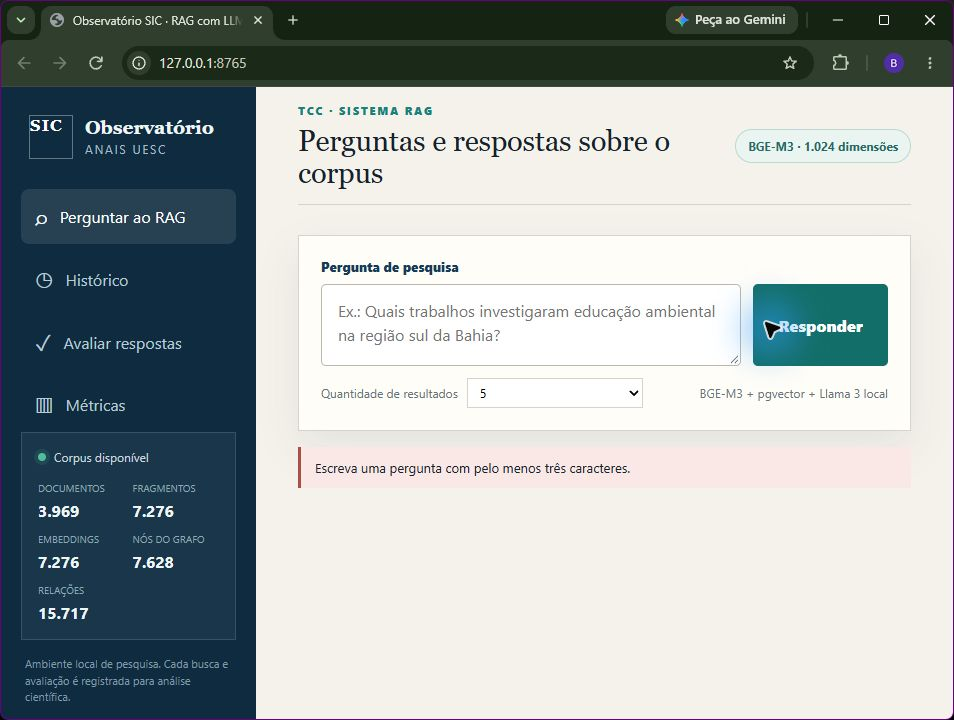
\includegraphics[width=\linewidth]{figuras/interface_consulta.png}
\par\smallskip
{\setstretch{1}\footnotesize\textbf{Fonte:} Elaborada pelo autor (2026).\par}
\end{minipage}
\end{figure}

A Figura~\ref{fig:interface-avaliacao} mostra a interface utilizada para comparar cada resposta com as fontes fornecidas ao modelo. O formulário mantém pergunta, resposta, evidências e critérios na mesma tela, reduzindo a necessidade de consultar registros externos durante o julgamento.

\begin{figure}[!htbp]
\centering
\begin{minipage}{0.96\textwidth}
\caption{Interface de avaliação humana das respostas geradas}
\label{fig:interface-avaliacao}
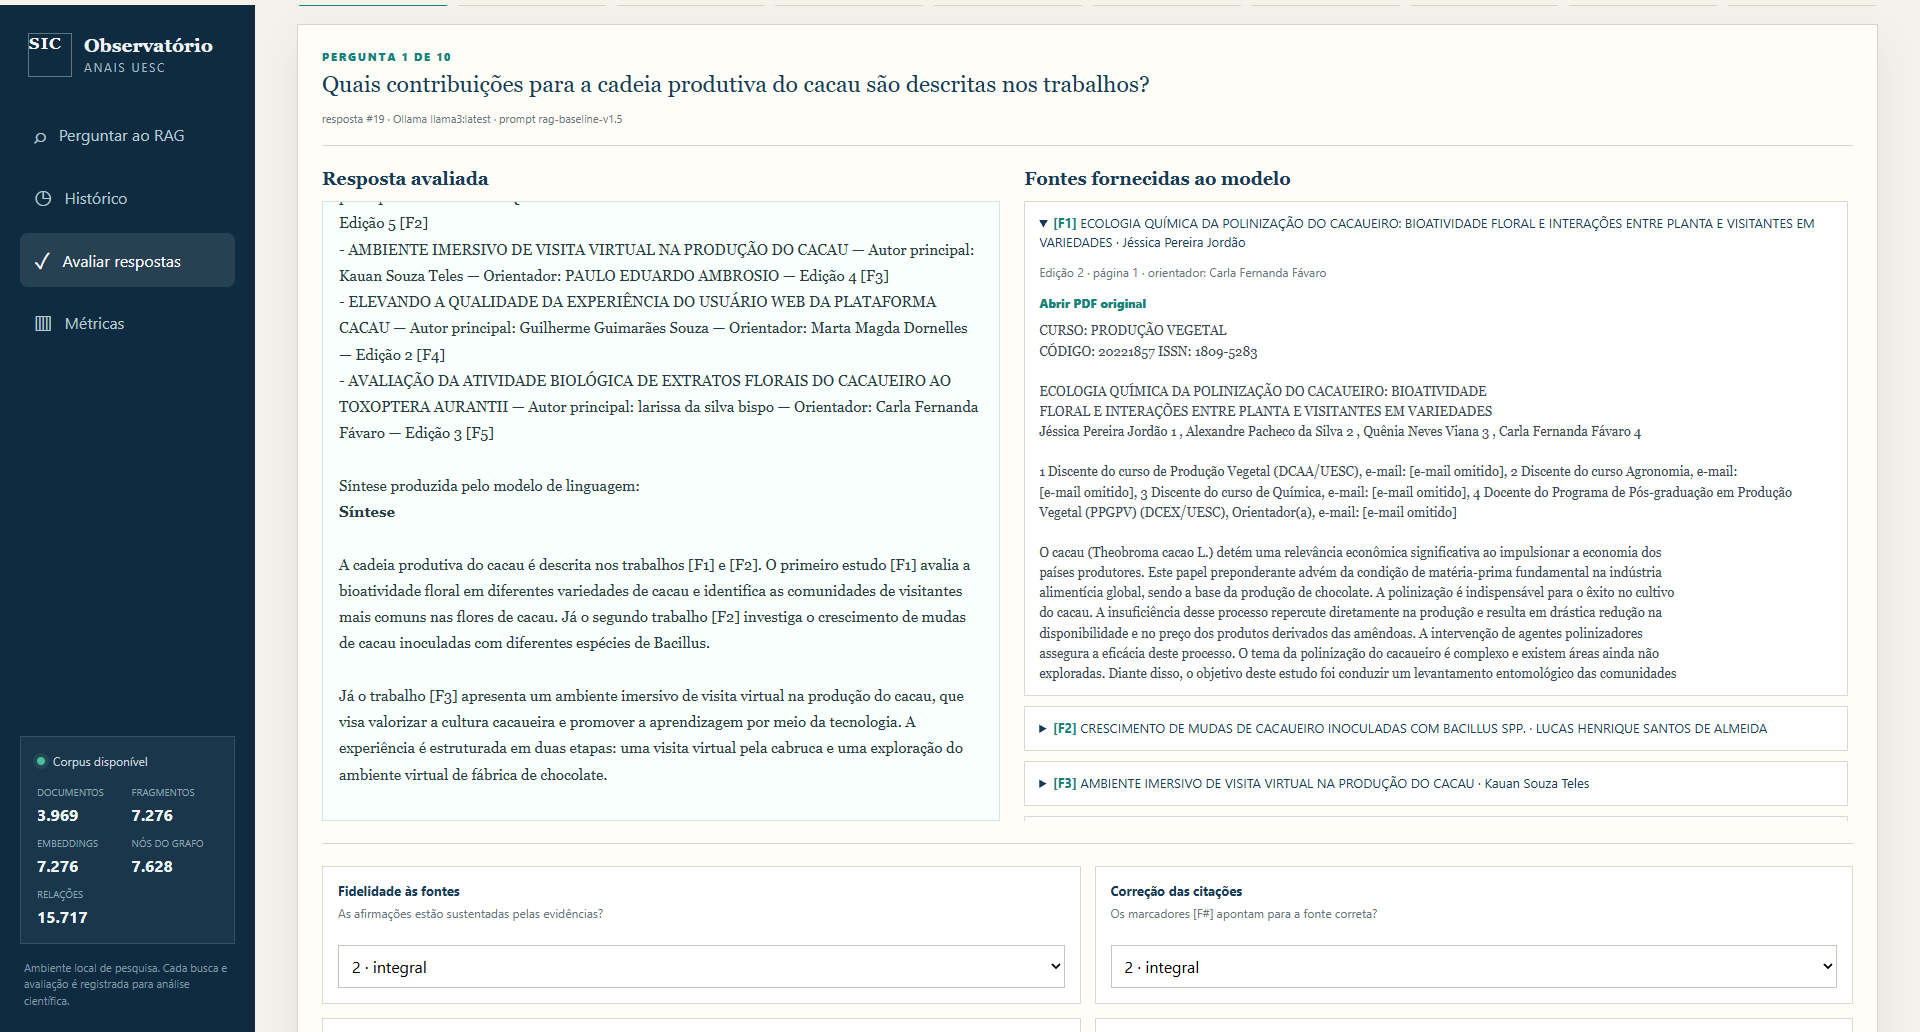
\includegraphics[width=\linewidth]{figuras/interface_avaliacao.png}
\par\smallskip
{\setstretch{1}\footnotesize\textbf{Fonte:} Elaborada pelo autor (2026), com dados de contato omitidos.\par}
\end{minipage}
\end{figure}

Em um teste sobre inteligência artificial com o \textit{prompt} \texttt{rag-baseline-v1.4}, o modelo confundiu nomes citados em um resumo com a autoria do trabalho. Na configuração \texttt{rag-baseline-v1.5}, a aplicação passou a montar o catálogo de fontes com título, autoria, orientação, edição e marcador. O modelo produz a síntese textual, cuja saída bruta permanece nos registros da execução.

A correção assegura que a identificação bibliográfica exibida não dependa da interpretação do modelo. A avaliação subsequente do conjunto congelado não identificou transferência temática entre fontes nas dez respostas examinadas. Esse resultado não elimina o risco, pois decorre de uma amostra pequena e de um único avaliador; por isso, a linha de base não é apresentada como solução definitiva.

\chapter{TECNOLOGIAS E BASE DE DADOS UTILIZADAS}

As escolhas tecnológicas foram orientadas por quatro requisitos do projeto: execução local, reprodutibilidade, rastreabilidade entre resposta e documento de origem e possibilidade de avaliação experimental. A arquitetura separa a preparação do corpus, a representação vetorial, a recuperação e a geração textual. Essa separação permite substituir um componente sem refazer toda a base e possibilita medir individualmente as etapas do RAG.

\section{Tecnologias empregadas}

A Tabela~\ref{tab:tecnologias-utilizadas} apresenta os principais componentes da implementação e sua função. As versões foram fixadas ou registradas nos artefatos para permitir a repetição das execuções.

O Python foi adotado por reunir bibliotecas maduras para processamento de documentos, aprendizado de máquina e construção de serviços. A vetorização com o BAAI/bge-m3 foi executada em CPU, com comprimento máximo de 1.024 \textit{tokens} e normalização dos vetores. O identificador completo da revisão, a biblioteca, a versão do \textit{framework}, o dispositivo e os parâmetros do modelo são armazenados na tabela de modelos de \textit{embedding}. Isso evita que o nome genérico do modelo seja a única informação disponível para reprodução.

O PostgreSQL foi escolhido como repositório central para manter, sob as mesmas restrições de integridade, os dados relacionais e as representações vetoriais. A extensão pgvector acrescenta o tipo \texttt{vector(1024)} e o operador de distância de cosseno, sem separar os vetores de sua proveniência documental. Na linha de base, a busca é exata: todos os 7.276 vetores compatíveis com o modelo são candidatos ao ordenamento, e os primeiros resultados são selecionados pelo menor valor de distância.

O Ollama mantém o processamento generativo no computador local. Essa decisão reduz a exposição do corpus a serviços externos e permite registrar o nome e o resumo criptográfico do modelo utilizado. A camada FastAPI organiza as requisições da interface, mas não contém o conhecimento do domínio: as evidências continuam armazenadas no banco e são fornecidas ao modelo somente durante cada consulta.

\begin{table}[!htbp]
\centering
\caption{Tecnologias utilizadas no sistema RAG}
\label{tab:tecnologias-utilizadas}
\renewcommand{\arraystretch}{1.18}
\small
\begin{tabularx}{\textwidth}{>{\raggedright\arraybackslash}p{3.1cm}>{\raggedright\arraybackslash}p{3.5cm}>{\raggedright\arraybackslash}X}
\toprule
\textbf{Componente} & \textbf{Versão ou configuração} & \textbf{Função no projeto} \\ \midrule
Python & 3.12.14 & Implementação dos procedimentos de auditoria, extração, segmentação, vetorização, recuperação e serviços da aplicação \cite{python}. \\
PowerShell & Ambiente nativo do Windows & Automação operacional, execução em lotes, inicialização dos serviços e acompanhamento por arquivos de log. \\
pypdf & 6.21.4, modo \texttt{layout} & Extração do conteúdo textual dos PDFs com preservação aproximada da organização visual e separação por página. \\
Sentence Transformers & 6.3.0, PyTorch 2.15.0 CPU & Carregamento e execução reproduzível do modelo BAAI/bge-m3 para codificação de perguntas e fragmentos. \\
BAAI/bge-m3 & Revisão \texttt{5617a9f...}; 1.024 dimensões & Produção de vetores densos multilíngues normalizados para representar semanticamente o corpus \cite{chen2024bgem3}. \\
PostgreSQL e pgvector & PostgreSQL 17.11; pgvector 0.8.7 & Persistência conjunta de metadados, textos, vetores e resultados; ordenação exata pela distância de cosseno \cite{postgresql,pgvector}. \\
FastAPI e Psycopg & FastAPI 0.121.2; Psycopg 3.2.12 & Exposição da interface local de busca, geração e avaliação, com acesso transacional ao PostgreSQL. \\
Ollama e Llama 3 & Ollama 0.40.16; \texttt{llama3:latest}, 8B, Q4\_0 & Execução local do modelo gerador. Não participa da geração dos \textit{embeddings}; recebe somente a pergunta e as fontes recuperadas. \\ \bottomrule
\end{tabularx}
\fontetabela{Elaborada pelo autor (2026).}
\end{table}
\section{Fonte, composição e delimitação do corpus}

A fonte documental é o portal público dos Anais da Semana de Iniciação Científica da UESC \cite{sicuescanais}. O recorte utilizado corresponde às edições 1 a 5 disponíveis no portal em novembro de 2026. A fotografia congelada do corpus contém 3.969 PDFs válidos e 3.970 páginas, posteriormente transformadas em 7.276 fragmentos textuais. O conjunto é utilizado como base externa de conhecimento do RAG e não como dados para treinamento ou ajuste dos parâmetros do Llama 3.

Cada documento é identificado pelo resumo SHA-256 de seus bytes. Para ele são preservados edição, identificador no portal, participante principal, caminho do arquivo, tamanho, quantidade de páginas, estado de auditoria e instante de processamento. Para cada página são mantidos texto bruto, texto normalizado, método e versão do extrator, métricas de qualidade, resumo criptográfico do texto e indicação de necessidade de OCR. Título e orientador são obtidos deterministicamente do cabeçalho da página quando a resposta é montada; não são inferidos livremente pela LLM.

Os endereços de e-mail existentes nos documentos não constituem campos de busca ou apresentação. Embora possam permanecer no texto documental necessário à auditoria, são omitidos do catálogo de fontes e o \textit{prompt} proíbe sua reprodução. A interface é acessível somente no ambiente local nesta etapa do projeto.

\section{Organização lógica da base de dados}

A modelagem foi dividida em cinco camadas relacionadas por chaves estrangeiras. A primeira reúne \texttt{documents} e \texttt{pages}, responsáveis pela proveniência e pelo texto extraído. A segunda reúne \texttt{chunks}, \texttt{embedding\_models} e \texttt{chunk\_embeddings}, que ligam cada vetor ao fragmento, à página, ao documento e à versão exata do modelo. A terceira contém \texttt{retrieval\_runs}, \texttt{retrieval\_results} e \texttt{relevance\_judgments}, preservando a pergunta, o vetor da consulta, o ranking, a distância de cosseno, os tempos medidos e o julgamento humano. A quarta reúne \texttt{generated\_answers} e \texttt{answer\_sources}, associando cada resposta às fontes numeradas efetivamente fornecidas ao gerador. A quinta contém os nós e as arestas da projeção do grafo de conhecimento, sempre vinculados aos documentos de origem.

A Figura~\ref{fig:der-banco-rag} apresenta o modelo entidade-relacionamento. PK indica chave primária, FK indica chave estrangeira e UK indica uma restrição de unicidade. Essas ligações preservam a proveniência de vetores, julgamentos e respostas. A resposta gerada permanece vinculada à execução, às evidências recuperadas e aos documentos de origem.

\begin{landscape}
\begin{figure}[p]
\centering
\begin{minipage}{0.96\linewidth}
\caption{Modelo entidade-relacionamento da base de dados do RAG}
\label{fig:der-banco-rag}
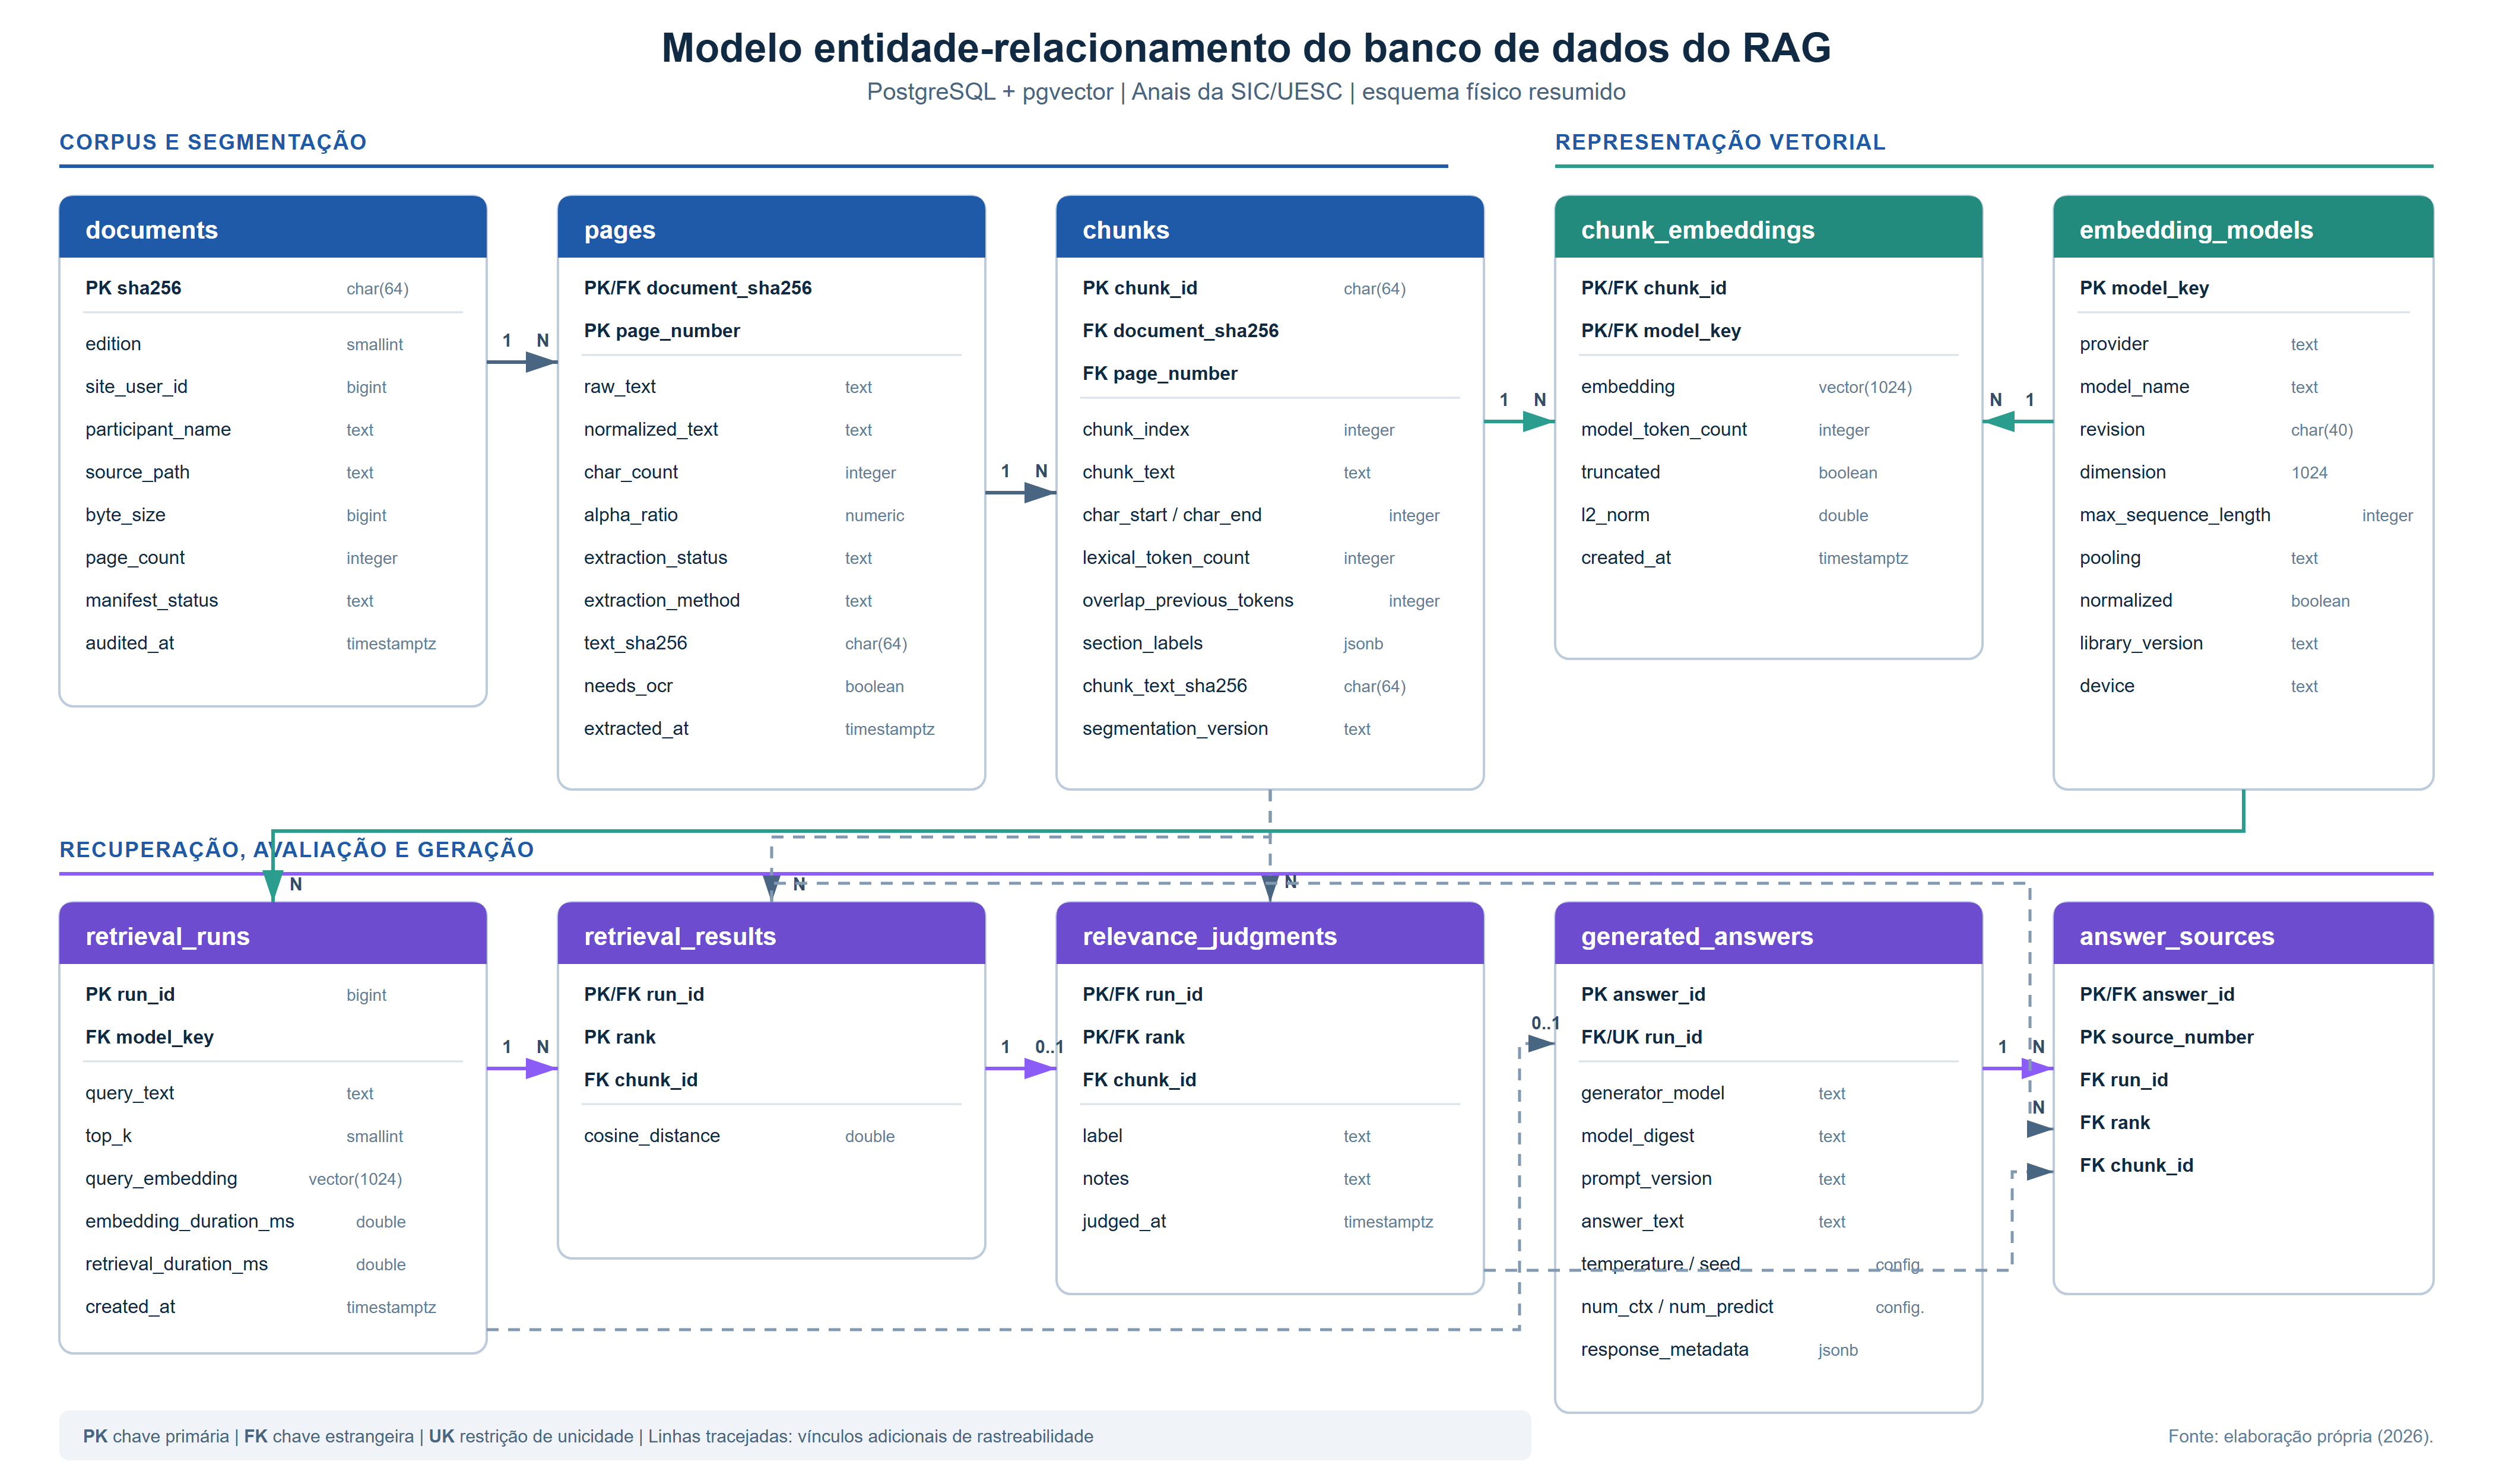
\includegraphics[width=\linewidth]{figuras/der_banco_rag_uesc.png}
\par\smallskip
{\setstretch{1}\footnotesize\textbf{Fonte:} Elaborada pelo autor (2026).\par}
\end{minipage}
\end{figure}
\end{landscape}

\section{Projeção do grafo de conhecimento}

A base foi ampliada com uma projeção de grafo de propriedades destinada a perguntas estruturais e agregadas que não devem ser respondidas pela recuperação de poucos fragmentos. Essa camada complementa a busca semântica: perguntas sobre o conteúdo dos trabalhos continuam sendo encaminhadas ao RAG vetorial, enquanto contagens e relações explícitas podem ser obtidas por consultas determinísticas. Nesta etapa, o grafo foi persistido no próprio PostgreSQL para manter metadados, vetores, nós, arestas e proveniência sob as mesmas transações e restrições de integridade, sem introduzir um segundo servidor.

Foram definidos quatro tipos de nó: \texttt{work}, para o trabalho identificado pelo SHA-256 do PDF; \texttt{person}, para participante principal ou orientador; \texttt{edition}, para as edições 1 a 5; e \texttt{course}, para o curso informado no cabeçalho. As arestas partem do trabalho e utilizam os tipos \texttt{AUTHORED\_BY}, \texttt{ADVISED\_BY}, \texttt{PRESENTED\_IN} e \texttt{ASSOCIATED\_WITH\_COURSE}. Cada aresta conserva o documento e a página de origem, de modo que uma relação possa ser rastreada até o PDF que a sustenta.

\begin{figure}[!htbp]
\centering
\begin{minipage}{\linewidth}
\caption{Modelo entidade-relacionamento da projeção do grafo de conhecimento}
\label{fig:der-grafo-conhecimento}
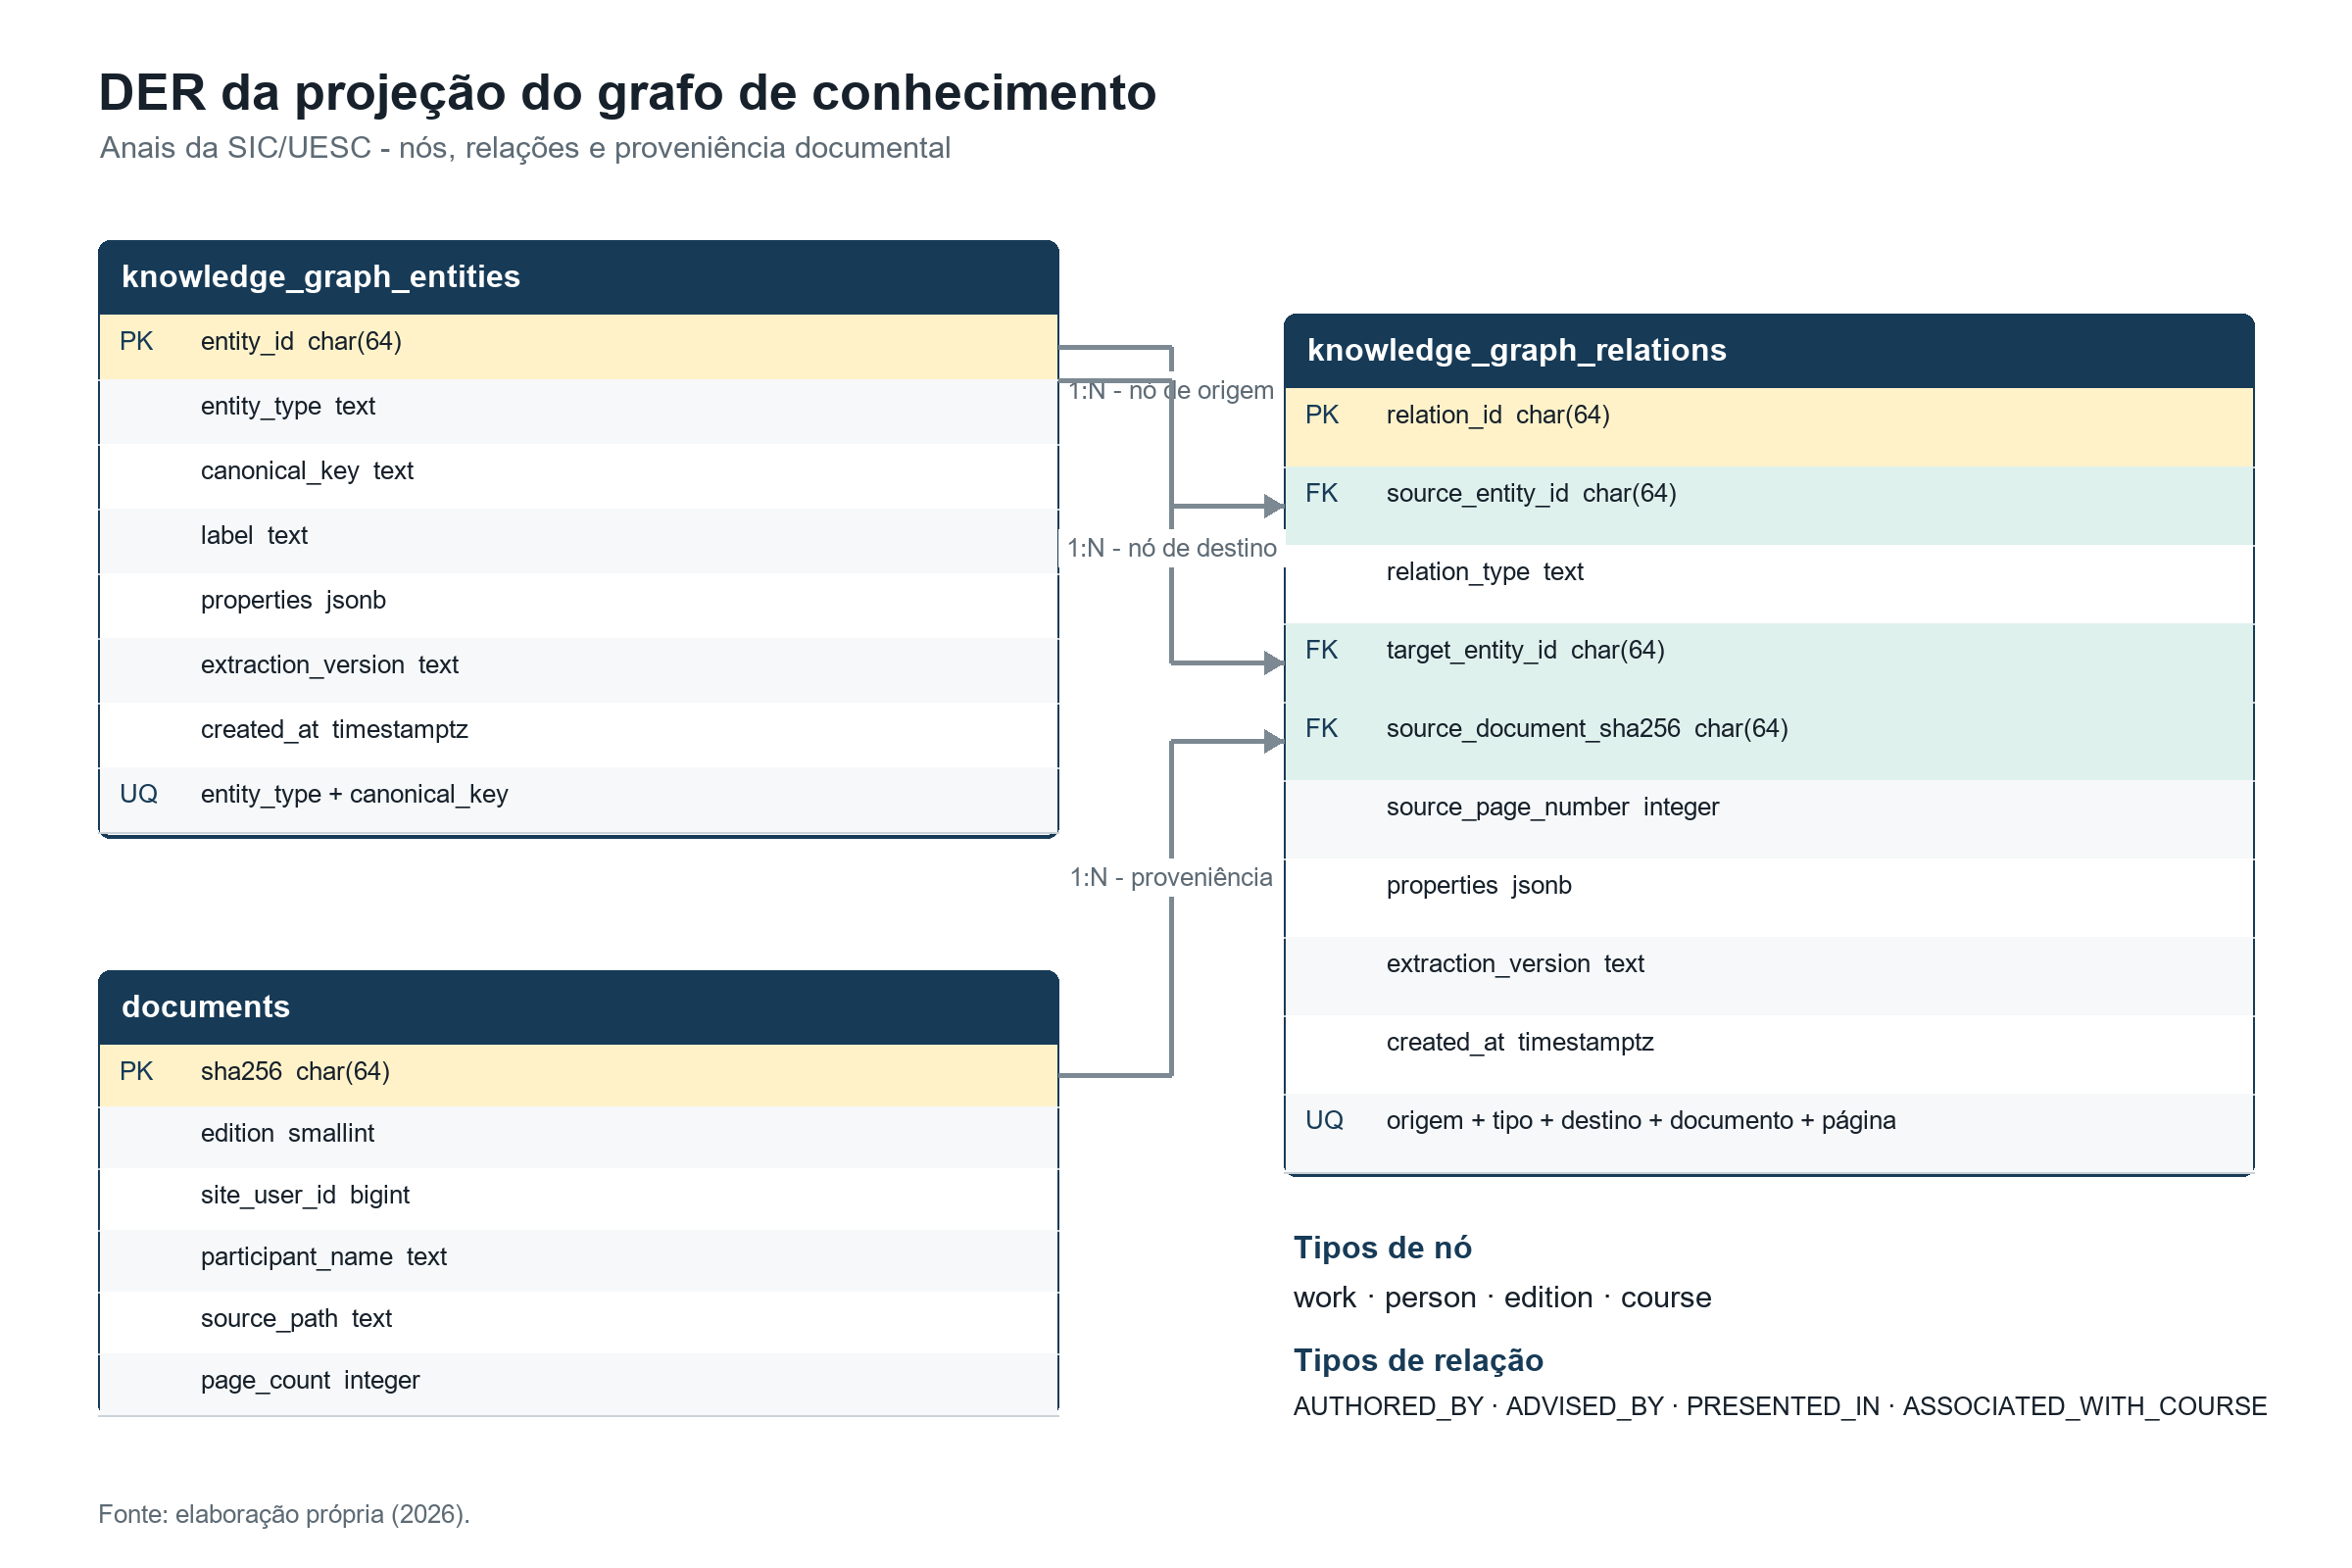
\includegraphics[width=\linewidth]{figuras/der_grafo_conhecimento.png}
\par\smallskip
{\setstretch{1}\footnotesize\textbf{Fonte:} Elaborada pelo autor (2026).\par}
\end{minipage}
\end{figure}

A Figura~\ref{fig:der-grafo-conhecimento} apresenta as tabelas implementadas. A tabela \path{knowledge_graph_entities} armazena os nós tipados, o rótulo de apresentação, a chave canônica, propriedades adicionais e a versão do extrator. A tabela \path{knowledge_graph_relations} armazena as arestas direcionadas, duas chaves estrangeiras para os nós de origem e destino e uma chave estrangeira para \texttt{documents}. A restrição de unicidade formada por origem, tipo, destino, documento e página impede a duplicação do mesmo vínculo proveniente da mesma evidência.

No DER, uma entidade pode participar de várias relações como origem ou destino, mas cada relação possui exatamente uma entidade de origem e uma de destino. Cada aresta também referencia um único documento, ao passo que um documento pode fundamentar várias relações. Essa cardinalidade permite representar, por exemplo, um trabalho ligado ao participante principal, ao orientador, à edição e ao curso, mantendo a proveniência de todos os vínculos. A chave estrangeira para \texttt{documents} integra o grafo à camada documental, e o SHA-256 do PDF funciona como identificador estável do trabalho em toda a arquitetura.

\subsection{Extração, normalização e carga}

O arquivo \path{src/rag_anais/graph_metadata.py} extrai os metadados da primeira página já armazenada na tabela \texttt{pages}. O procedimento localiza o participante principal a partir do metadado do portal, considera como título as linhas entre o código do trabalho e o bloco de autoria, lê o campo \texttt{CURSO:} e associa a numeração do bloco de autores à afiliação marcada como \textit{Orientador(a)}. Nenhuma relação de orientação é inferida pela LLM. Quando o marcador explícito não é encontrado, a aresta permanece ausente e o documento é registrado para revisão.

Nomes de pessoas e cursos são transformados em chaves canônicas por normalização de caixa, acentuação e espaços, enquanto o rótulo original é preservado para apresentação. O identificador de cada nó é um SHA-256 determinístico do tipo e da chave canônica. O identificador de cada aresta é calculado a partir da origem, do tipo, do destino e do documento de proveniência. Essa estratégia torna a carga idempotente: as mesmas entradas produzem os mesmos identificadores em novas execuções.

Antes da carga integral, quatro documentos de cada edição foram auditados, totalizando vinte registros. A amostra apresentou título, orientador e curso identificados em todos os casos. Em seguida, o programa \path{scripts/build_knowledge_graph.py} processou os 3.969 documentos em modo de prévia. A cobertura foi de 100,00\% para título, 99,90\% para orientador e 96,09\% para curso. Quatro documentos não apresentaram orientador identificável e 155 não apresentaram curso no formato reconhecido. Esses casos foram mantidos com relações parciais e preservados em \path{artifacts/knowledge_graph/knowledge_graph_warnings.csv}, sem preenchimento especulativo.

A gravação integral foi realizada em uma única transação com a versão \texttt{graph-metadata-v1}. A Tabela~\ref{tab:grafo-contagens} apresenta as quantidades produzidas.

\begin{table}[htbp]
\centering
\caption{Nós e relações da projeção do grafo de conhecimento}
\label{tab:grafo-contagens}
\renewcommand{\arraystretch}{1.18}
\small
\begin{tabular*}{\textwidth}{@{\extracolsep{\fill}}lrlr}
\toprule
\textbf{Tipo de nó} & \textbf{Quantidade} & \textbf{Tipo de relação} & \textbf{Quantidade} \\ \midrule
Trabalho & 3.969 & \texttt{AUTHORED\_BY} & 3.969 \\
Pessoa & 3.594 & \texttt{ADVISED\_BY} & 3.965 \\
Curso & 60 & \texttt{PRESENTED\_IN} & 3.969 \\
Edição & 5 & \texttt{ASSOCIATED\_WITH\_COURSE} & 3.814 \\ \bottomrule
\end{tabular*}
\fontetabela{Dados da carga do grafo de conhecimento (2026).}
\end{table}

\subsection{Roteamento e busca híbrida}

A projeção foi integrada à aplicação por meio do arquivo \path{src/rag_anais/graph_queries.py}. A função de roteamento normaliza a pergunta, identifica marcadores de agregação e extrai, quando presentes, nomes de autor, orientador, curso ou edição. A decisão é registrada com a versão \texttt{query-router-v1.2} e conduz a uma das três rotas a seguir:

\begin{enumerate}
    \item \textbf{estrutural}: utilizada para listas, contagens, rankings e relações explícitas. A resposta é montada diretamente a partir de consultas SQL parametrizadas sobre os nós e as arestas;
    \item \textbf{semântica}: utilizada quando a pergunta solicita temas, métodos, resultados ou outras evidências presentes no texto. Nesse caso, a recuperação vetorial continua sendo executada sobre o corpus integral;
    \item \textbf{híbrida}: utilizada quando a pergunta combina uma entidade estruturada com uma necessidade de informação textual, como ``quais trabalhos orientados por uma pessoa tratam de cacau?''.
\end{enumerate}

Na rota híbrida, o grafo atua primeiro como filtro. A entidade citada é localizada por sua chave canônica e suas arestas produzem a lista de SHA-256 dos documentos permitidos. Essa lista é entregue ao recuperador do arquivo \path{src/rag_anais/web_app.py}, que calcula o \textit{embedding} da pergunta com o modelo BGE-M3 e executa a busca por similaridade de cosseno no pgvector somente dentro desse subconjunto. Os fragmentos recuperados e ordenados formam o contexto enviado ao Llama~3 por meio do Ollama. Assim, o grafo define corretamente o universo documental, enquanto o recuperador semântico localiza as passagens relevantes e a LLM redige a resposta fundamentada.

O fluxo pode ser resumido como: pergunta $\rightarrow$ classificação da intenção $\rightarrow$ filtro relacional no grafo $\rightarrow$ recuperação vetorial restrita $\rightarrow$ montagem do contexto $\rightarrow$ geração da resposta. A separação é importante porque a LLM não deve estimar contagens nem inventar relações. Consultas quantitativas são calculadas pelo PostgreSQL; a LLM participa apenas quando há síntese de conteúdo textual. Cada execução é auditada em \texttt{query\_route\_runs}, que conserva rota, intenção, justificativa, versão do roteador, consulta executada, quantidade de documentos no escopo e duração. Isso permite reproduzir a decisão do sistema e comparar versões posteriores.

\subsection{Validação funcional do grafo e do roteamento}

O programa \path{scripts/validate_knowledge_graph.py} confirmou que os 3.969 documentos correspondem a 3.969 nós de trabalho. Cada trabalho possui uma relação de autoria principal e uma relação de edição. A verificação também confirmou a ausência de arestas órfãs e a correspondência entre as contagens por edição e o corpus auditado.

Em 21 de novembro de 2026, o roteador classificou corretamente as cinco perguntas da Tabela~\ref{tab:validacao-grafo-estrutural} como estruturais. O PostgreSQL produziu as respostas de forma determinística, com tempo médio de 11,86\,ms no ambiente local.

\begin{table}[!htbp]
\centering
\caption{Resultados da validação das consultas estruturais}
\label{tab:validacao-grafo-estrutural}
\small
\setlength{\tabcolsep}{5pt}
\renewcommand{\arraystretch}{1.12}
\begin{tabularx}{\textwidth}{>{\raggedright\arraybackslash}p{0.43\textwidth}>{\raggedright\arraybackslash}X}
\toprule
\textbf{Pergunta} & \textbf{Resultado} \\ \midrule
Quais foram os trabalhos apresentados por Breno Gonçalves Pirôpo? & \textit{Radar de Furto e Roubo de Veículos Automotores} (edição 4) e \textit{ConectCacau} (edição 5). \\
Quais trabalhos foram orientados por Gesil Sampaio Amarante Segundo? & 28 trabalhos nas edições 1 a 3, entre eles \textit{Preparação de conteúdos para o CDC-UESC}. \\
Quais trabalhos estão relacionados ao curso de Ciência da Computação? & 124 trabalhos, entre eles \textit{Gestão inteligente de água}. \\
Quantos trabalhos foram apresentados em cada edição da SIC/UESC? & Da edição 1 à 5, respectivamente: 680, 973, 733, 754 e 829. Total de 3.969 trabalhos. \\
Quais cursos apresentam mais trabalhos? & Enfermagem (288), Biomedicina (282) e Medicina Veterinária (276) lideram o ranking. \\ \bottomrule
\end{tabularx}
\fontetabela{Dados da validação funcional do grafo (2026).}
\end{table}

A verificação do roteamento, executada por \path{scripts/validate_graph_query_integration.py}, registrou 24 execuções sem erro. Na pergunta sobre cacau na edição 3, a rota híbrida limitou a busca vetorial aos 733 documentos da edição e retornou cinco resultados. Os resumos de carga e integridade e as respostas completas, com fontes e tempos individuais, constam em \path{artifacts/knowledge_graph/}, nos arquivos \path{knowledge_graph_build_summary.json}, \path{knowledge_graph_validation.json} e \path{experimento_grafo_5_perguntas.json}.

Os resultados descrevem a integridade do grafo e o funcionamento das rotas. A qualidade das respostas estruturais e híbridas permanece como objeto de avaliação humana futura. A consolidação por nome normalizado agrupou variações de grafia ou caixa em 343 chaves de pessoa. Homônimos podem exigir revisão dos vínculos no documento de origem.


\section{Persistência, auditoria e reprodutibilidade}

A implementação foi organizada para que a preparação do corpus e a execução do RAG possam ser repetidas sem depender de operações manuais não documentadas. O diretório-raiz da aplicação é \path{rag_anais_uesc}; os PDFs congelados permanecem em \path{D:\tcc_sic}, separados por edição. A reprodução numérica exata pressupõe o uso dos mesmos PDFs, do manifesto preservado e das revisões de modelos registradas, pois uma nova coleta feita após alterações no portal pode produzir um corpus diferente. O ambiente utilizado emprega Windows 11, PowerShell, Python 3.12.14, Docker Desktop, PostgreSQL 17.11, pgvector 0.8.7 e Ollama 0.40.16.

\subsection{Arquivos e ordem de reprodução}

A reprodução segue a sequência de coleta e auditoria dos PDFs, extração textual, segmentação, auditoria do limite do tokenizador, geração de vetores, carga no PostgreSQL e construção da projeção em grafo. A extração integral é executada por \path{src/rag_anais/extract_corpus.py}, com pypdf 6.21.4 em modo \texttt{layout}. Os parâmetros de segmentação são alvo de 450 unidades lexicais, máximo de 520, mínimo desejado de 120 e sobreposição desejada de 75.

A indexação e a consulta empregam a mesma revisão do BAAI/bge-m3, com vetores normalizados de 1.024 dimensões e limite de 1.024 \textit{tokens}. Na avaliação da linha de base, a recuperação por cosseno utiliza \textit{top-k} igual a 5. A geração utiliza \texttt{llama3:latest}, com o \textit{prompt} \texttt{rag-baseline-v1.5}, temperatura 0, semente 42, contexto de 8.192 \textit{tokens} e limite de 700 \textit{tokens} de saída. As verificações incluem a integridade dos PDFs, a ausência de truncamento e a correspondência entre documentos, páginas, fragmentos e vetores.

O \href{https://github.com/BrenoPiropo/tcc_rag/blob/main/README.md}{\texttt{README.md} do repositório \texttt{tcc\_rag}} documenta os pré-requisitos, os comandos, a ordem de execução dos arquivos e os critérios de validação. A implementação de referência está identificada pelo \href{https://github.com/BrenoPiropo/tcc_rag/tree/2b1bb15cd4d6d9fb433c50de21f32d0dc04f6e6d}{commit \texttt{2b1bb15}}. O protocolo registra as revisões dos modelos, o resumo criptográfico do manifesto e os artefatos necessários para conferir a reprodução.

\subsection{Evidências de auditoria}

Os arquivos em \path{artifacts/} constituem as evidências reprodutíveis de cada etapa. Os resumos \path{corpus_audit.json}, \path{corpus_extraction_summary.json}, \path{corpus_segmentation_summary.json}, \path{embedding_token_audit.json} e \path{corpus_embeddings_summary.json} registram contagens, parâmetros, versões, durações e resumos criptográficos das entradas. Os arquivos \path{corpus_extraction_db_validation.json}, \path{corpus_segmentation_db_validation.json} e \path{corpus_embeddings_db_validation.json} preservam as verificações realizadas depois de cada carga. A validação da interface está em \path{web_interface_validation_2026-11-13.json}, e a validação do RAG com LLM está em \path{rag_llm_baseline_validation_2026-11-13.json}. Os logs independentes permitem acompanhar o processamento sem depender da interface.

Cada consulta recebe um \texttt{run\_id}. São preservados a pergunta, o modelo de \textit{embedding}, o \textit{top-k}, o vetor da consulta, os fragmentos ordenados, as distâncias de cosseno e os tempos de vetorização e recuperação. Para a geração também são armazenados provedor, nome e resumo do modelo, versão e SHA-256 do \textit{prompt}, temperatura, semente, janela de contexto, limite de saída, duração, resposta, metadados brutos e fontes numeradas. Assim, uma resposta pode ser reconstruída desde o texto exibido até o fragmento, a página, o PDF e a configuração exata dos modelos utilizados.

\chapter{RESULTADOS E DISCUSSÃO}

O corpus integral foi coletado e auditado. As edições 1 a 5 totalizam 3.969 PDFs válidos e 3.970 páginas. O manifesto final da edição 5 contém 829 documentos, um a menos que a contagem preliminar de formulários; o relatório conserva ambos os valores e utiliza somente os arquivos efetivamente auditados nos resultados. A Tabela~\ref{tab:mapeamento} apresenta a distribuição dos documentos e fragmentos efetivamente indexados.

\begin{table}[htbp]
\centering
\caption{Corpus validado e fragmentos indexados por edição}
\label{tab:mapeamento}
\renewcommand{\arraystretch}{1.2}
\begin{tabular*}{\textwidth}{@{\extracolsep{\fill}}cccc}
\toprule
\textbf{Edição} & \textbf{Ano} & \textbf{PDFs válidos} & \textbf{Fragmentos} \\ \midrule
1 & 2022 & 680 & 1.199 \\
2 & 2023 & 973 & 1.739 \\
3 & 2024 & 733 & 1.352 \\
4 & 2025 & 754 & 1.414 \\
5 & 2026 & 829 & 1.572 \\
\textbf{Total} & 2022--2026 & \textbf{3.969} & \textbf{7.276} \\ \bottomrule
\end{tabular*}
\fontetabela{Dados da pesquisa (2026).}
\end{table}

A extração integral foi concluída em 336,703 segundos e não produziu página vazia, erro ou candidato a OCR. A segmentação gerou 7.276 fragmentos, todos cobertos por 7.276 \textit{embeddings} normalizados de 1.024 dimensões. A geração integral dos vetores foi executada localmente, em CPU, e não apresentou truncamento, duplicidade de identificador ou vetor órfão.

No banco, uma consulta exata pelos dez vizinhos mais próximos apresentou 32,003 e 38,246 milissegundos em duas medições técnicas iniciais. Na validação da interface, com o modelo já residente em memória, uma pergunta controlada levou 135,03 milissegundos para ser vetorizada e 70,44 milissegundos para a recuperação exata. Esses valores descrevem o ambiente local e não constituem, isoladamente, uma avaliação de qualidade.

A interface e a linha de base com LLM foram validadas de ponta a ponta. O teste final do \textit{pipeline} utilizou cinco fontes, 4.143 \textit{tokens} de entrada e 518 \textit{tokens} gerados; a geração levou 12.791,28 milissegundos. A persistência da resposta, das fontes, dos parâmetros e dos tempos foi confirmada. A correção determinística dos metadados solucionou o erro de autoria observado no catálogo, mas a síntese ainda requer avaliação por poder confundir conteúdos entre fontes.

\section{Perguntas do experimento temático}

As dez perguntas abaixo compõem o conjunto do experimento temático e orientaram os julgamentos humanos sobre a relevância das fontes e a qualidade das respostas.

\begin{enumerate}
    \item Quais contribuições para a cadeia produtiva do cacau são descritas nos trabalhos?
    \item Quais aplicações de inteligência artificial aparecem nos Anais?
    \item Que problemas ambientais do sul da Bahia são investigados?
    \item Quais temas de saúde pública aparecem nos trabalhos?
    \item Como a agricultura familiar é abordada nas pesquisas?
    \item Quais estudos tratam da biodiversidade regional?
    \item Que metodologias de ensino são relatadas nos trabalhos de educação?
    \item Quais soluções de inovação tecnológica foram desenvolvidas na UESC?
    \item Como questões de gênero, raça e inclusão social aparecem nas pesquisas?
    \item Quais relações interdisciplinares podem ser identificadas entre trabalhos de áreas diferentes?
\end{enumerate}

Essas consultas exigem recuperação de evidências textuais. Perguntas quantitativas, como a quantidade de trabalhos por curso ou edição, foram respondidas por consultas estruturadas aos metadados e não pela geração de texto baseada em poucos trechos.

Foram alcançados o corpus validado, a extração textual integral, a segmentação auditável, a geração de todos os \textit{embeddings}, o armazenamento no pgvector, a recuperação semântica exata, a interface de avaliação e uma linha de base RAG com modelo de linguagem local. A aplicação permite abrir o PDF correspondente, examinar a evidência utilizada e registrar julgamentos humanos.

\section{Experimento temático}

A linha de base foi avaliada com as dez perguntas temáticas da seção anterior. O BAAI/bge-m3 representou cada pergunta como um vetor, e o pgvector selecionou os cinco fragmentos mais próximos entre os 7.276 indexados. O modelo local \texttt{llama3:latest} recebeu as páginas correspondentes após a remoção de fontes duplicadas. As execuções de 13 de novembro de 2026 (identificadores 15 a 24) e as respectivas respostas foram preservadas no PostgreSQL.

\subsection{Uso da similaridade de cosseno}

Para o vetor da pergunta $\mathbf{q}$ e o vetor do fragmento $\mathbf{d}_{i}$, a similaridade foi calculada a partir da distância retornada pelo pgvector:

\begin{equation}
\operatorname{sim}(\mathbf{q},\mathbf{d}_{i}) = 1 - \operatorname{dist}_{\cos}(\mathbf{q},\mathbf{d}_{i}).
\end{equation}

A pontuação ordena os fragmentos por proximidade semântica estimada. A Figura~\ref{fig:similaridade-cosseno} apresenta sua interpretação geométrica, e a Tabela~\ref{tab:resultados-experimento-tematico} registra os valores nas cinco primeiras posições. A relevância dos fragmentos e a qualidade das respostas foram julgadas separadamente.

\begin{figure}[!htbp]
\centering
\begin{minipage}{0.90\textwidth}
\caption{Interpretação geométrica da similaridade de cosseno}
\label{fig:similaridade-cosseno}
\resizebox{\linewidth}{!}{%
\begin{tikzpicture}[font=\small, scale=1.0]
  \draw[->, line width=0.7pt] (0,0) -- (7.2,0) node[right] {dimensão 1};
  \draw[->, line width=0.7pt] (0,0) -- (0,4.8) node[above] {dimensão 2};
  \draw[-{Latex[length=2.6mm]}, line width=1.2pt, draw=blue!70!black] (0,0) -- (5.8,2.1) node[right, text=black] {$\mathbf{d}_{i}$};
  \draw[-{Latex[length=2.6mm]}, line width=1.2pt, draw=orange!80!black] (0,0) -- (3.1,4.0) node[above, text=black] {$\mathbf{q}$};
  \draw[draw=black!70, line width=0.7pt] (1.35,0.49) arc[start angle=20,end angle=52,radius=1.43];
  \node at (1.55,1.05) {$\theta$};
  \node[resultbox, text width=5.8cm] at (10.4,2.5) {$\displaystyle \operatorname{sim}(\mathbf{q},\mathbf{d}_{i})=\cos(\theta)=\frac{\mathbf{q}\cdot\mathbf{d}_{i}}{\lVert\mathbf{q}\rVert\,\lVert\mathbf{d}_{i}\rVert}$\\[3pt]Ângulo menor $\Rightarrow$ maior similaridade};
\end{tikzpicture}
}
\par\smallskip
{\setstretch{1}\footnotesize\raggedright\textbf{Fonte:} Adaptada de \cite{manning2008ir}.\par}
\end{minipage}
\end{figure}

\subsection{Avaliação humana da recuperação}

Um avaliador julgou os vinte primeiros fragmentos de cada pergunta, totalizando 200 julgamentos. As classes foram \textbf{relevante} (evidência diretamente útil), \textbf{parcialmente relevante} (evidência indireta ou insuficiente) e \textbf{não relevante} (sem evidência útil). Somente a primeira classe entrou no cálculo de Recall@$5$ e MRR.

O Recall@$5$ condicionado ao \textit{pool}@20 divide o número de itens relevantes no \textit{top-5} pelo total de relevantes encontrados nas vinte primeiras posições do mesmo recuperador. Na análise documental, cada trabalho foi contado uma vez por pergunta e por corte quando continha pelo menos um fragmento relevante. O denominador representa o conjunto julgado, com cobertura restrita às vinte primeiras posições.

\begin{table}[!htbp]
\centering
\caption{Similaridade de cosseno e Recall@$5$ condicionado ao \textit{pool}@20}
\label{tab:resultados-experimento-tematico}
\setlength{\tabcolsep}{4pt}
\renewcommand{\arraystretch}{1.18}
\footnotesize
\begin{tabular*}{\textwidth}{@{\extracolsep{\fill}}c*{5}{c}cccc}
\toprule
\textbf{Nº} & \multicolumn{5}{c}{\textbf{Cosseno por posição (\%)}} & \multicolumn{2}{c}{\textbf{Fragmentos}} & \multicolumn{2}{c}{\textbf{Documentos}} \\
& \textbf{1º} & \textbf{2º} & \textbf{3º} & \textbf{4º} & \textbf{5º} & \textbf{Relev.} & \textbf{Recall@$5$} & \textbf{Relev.} & \textbf{Recall@$5$} \\ \midrule
1 & 60,47 & 60,16 & 59,85 & 59,44 & 59,32 & 5/16 & $0{,}3125$ & 5/16 & $0{,}3125$ \\
2 & 55,28 & 54,06 & 53,97 & 53,62 & 53,56 & 5/9 & $0{,}5556$ & 5/8 & $0{,}6250$ \\
3 & 61,97 & 59,20 & 57,86 & 57,62 & 56,82 & 4/8 & $0{,}5000$ & 4/8 & $0{,}5000$ \\
4 & 57,72 & 56,87 & 55,26 & 54,95 & 54,74 & 2/14 & $0{,}1429$ & 2/13 & $0{,}1538$ \\
5 & 61,20 & 59,43 & 59,29 & 59,12 & 58,78 & 5/13 & $0{,}3846$ & 5/12 & $0{,}4167$ \\
6 & 55,49 & 55,12 & 55,11 & 55,07 & 55,02 & 4/13 & $0{,}3077$ & 4/13 & $0{,}3077$ \\
7 & 61,75 & 61,16 & 61,00 & 60,88 & 60,83 & 3/9 & $0{,}3333$ & 3/8 & $0{,}3750$ \\
8 & 61,95 & 61,80 & 61,32 & 61,23 & 58,55 & 5/11 & $0{,}4545$ & 3/9 & $0{,}3333$ \\
9 & 62,98 & 61,26 & 61,19 & 59,99 & 59,64 & 5/20 & $0{,}2500$ & 5/18 & $0{,}2778$ \\
10 & 57,83 & 57,48 & 57,22 & 56,46 & 56,23 & 5/19 & $0{,}2632$ & 5/16 & $0{,}3125$ \\ \bottomrule
\end{tabular*}
\par\smallskip
\begin{minipage}{\textwidth}
\setstretch{1}\footnotesize\textbf{Nota:} Relev. mostra a contagem de itens relevantes no \textit{top-5} sobre a contagem no \textit{pool}@20.\\
\textbf{Fonte:} Dados da avaliação humana realizada pelo autor (2026).
\end{minipage}
\end{table}

O Recall@$5$ médio por pergunta foi de $0{,}3504$ por fragmento e $0{,}3614$ por documento. Na agregação das contagens por pergunta, os valores foram $0{,}3258$ (43 de 132 fragmentos) e $0{,}3388$ (41 de 121 documentos). O MRR foi $1{,}0000$ nos dois níveis, pois o primeiro resultado de cada pergunta foi relevante. O MRR informa a posição da primeira evidência. O Recall@$5$ mede a cobertura das evidências até a quinta posição.

Na pergunta sobre saúde pública (nº 4), apenas dois dos quatorze fragmentos relevantes apareceram nas cinco primeiras posições. As similaridades da quinta e da sexta posição foram $0{,}5474$ e $0{,}5437$, respectivamente. Evidências sobre hanseníase em Ilhéus e atendimento em Libras ficaram além do corte. Na pergunta sobre inovação tecnológica (nº 8), cinco fragmentos relevantes correspondiam a apenas três trabalhos. A deduplicação ocorreu depois da recuperação, sem reposição, e a LLM recebeu três fontes distintas. O Recall@$5$ caiu de $0{,}4545$ por fragmento para $0{,}3333$ por documento. O ensaio utilizou uma única configuração de deduplicação, o que limita a interpretação de seu efeito sobre as respostas.

\subsection{Avaliação humana da geração}

O mesmo avaliador comparou as dez respostas com as páginas fornecidas ao modelo, com cinco fontes em nove perguntas e três na pergunta 8. As respostas avaliadas (identificadores 19, 20 e 22 a 29) usaram o \textit{prompt} \texttt{rag-baseline-v1.5}. A escala de 0 a 2 representou falha importante, atendimento parcial e atendimento integral. As dez respostas receberam nota 2 em fidelidade às fontes, correção das citações, completude em relação ao contexto e separação entre fontes. Na pergunta 8, a resposta apresentou três trabalhos e o registro indicava uma recusa adequada. Essa inconsistência levou à exclusão do campo de recusa da interpretação.

A avaliação da geração descreve o aproveitamento das fontes disponibilizadas, enquanto a avaliação da recuperação mede a cobertura no conjunto julgado. A amostra de dez perguntas, a participação de um único avaliador e a possibilidade de evidências fora do \textit{pool}@20 limitam a generalização a outros acervos e modelos. Os julgamentos, as respostas e os parâmetros foram preservados no PostgreSQL e nos artefatos do experimento.


\chapter{CONCLUSÃO}

Este trabalho partiu da constatação de que, embora a Universidade Estadual de Santa Cruz disponha de um acervo científico expressivo nos Anais da Semana de Iniciação Científica, a consulta e a exploração integrada desse conteúdo ainda são limitadas pela forma como os documentos são disponibilizados. Os trabalhos podem ser acessados individualmente, mas a ausência de mecanismos que permitam formular perguntas em linguagem natural dificulta a identificação de temas, pesquisadores, orientadores, cursos e relações existentes no conjunto documental.

Diante desse cenário, foi desenvolvida uma plataforma destinada a ampliar o acesso às pesquisas realizadas na Universidade. A ferramenta permite transformar documentos dispersos em informações consultáveis e rastreáveis, podendo auxiliar estudantes, pesquisadores, gestores institucionais e agentes do setor produtivo na identificação de trabalhos, áreas de conhecimento e competências científicas presentes na UESC. A análise do corpus também evidenciou a diversidade temática das pesquisas produzidas nas edições estudadas e seu potencial para apoiar novas investigações, colaborações acadêmicas e aproximações entre a Universidade e a sociedade.

Para alcançar esse resultado, foi implementada uma arquitetura reproduzível de recuperação e síntese de informações dos Anais da SIC/UESC. O processo compreendeu coleta, auditoria, extração textual, segmentação, geração de \textit{embeddings}, persistência no PostgreSQL com pgvector, recuperação semântica, geração local com modelo de linguagem, projeção em grafo, interface de consulta e registro das execuções. A associação entre documentos, páginas, fragmentos, vetores, execuções, respostas e fontes preservou a proveniência necessária para verificar os resultados apresentados pelo sistema.

Na avaliação humana da recuperação, o MRR de 1,0000 indicou que o primeiro resultado das dez consultas foi considerado relevante. Entretanto, a saturação dessa métrica não informa a cobertura das posições seguintes. O macro Recall@$5$ condicionado ao \textit{pool}@20 foi de 0,3504 no nível de fragmento e de 0,3614 no nível de documento, demonstrando que as cinco primeiras posições recuperaram apenas parte das evidências relevantes identificadas até a vigésima posição. Esses resultados indicam que o principal aspecto a ser aprimorado na linha de base é a cobertura do ranking, especialmente em perguntas amplas que envolvem diversos trabalhos.

Na avaliação da geração, o avaliador atribuiu a pontuação máxima às dez respostas nos quatro critérios considerados: fidelidade às fontes, correção das citações, completude em relação ao contexto fornecido e separação entre documentos. Esse resultado, contudo, deve ser interpretado como evidência inicial, pois o experimento utilizou um número reduzido de perguntas e contou com apenas um avaliador. Portanto, não permite generalizar o desempenho do componente gerador para todas as possíveis consultas ao corpus.

A projeção em grafo complementou a recuperação semântica ao permitir consultas que exigem relações explícitas ou agregações sobre o conjunto de dados. As cinco perguntas estruturadas foram executadas de maneira determinística, e o roteador passou a distinguir consultas semânticas, estruturadas e híbridas.

Conclui-se que o sistema atende ao objetivo de disponibilizar uma plataforma rastreável para consulta aos Anais da SIC/UESC em linguagem natural. Os resultados demonstram a complementaridade entre a recuperação vetorial, adequada à localização de conteúdos semanticamente relacionados, e a representação em grafo, apropriada para perguntas sobre autores, orientadores, cursos, edições e quantidades. Além de estabelecer uma referência experimental reproduzível, o trabalho preserva os artefatos necessários para avaliar novas versões e contribui para tornar o conhecimento científico produzido na UESC mais acessível, consultável e útil para a comunidade acadêmica e para a sociedade.

\section{Projetos futuros}

Como continuidade deste trabalho, propõe-se aprimorar a recuperação de evidências, a geração de respostas e a representação em grafo dos Anais da Semana de Iniciação Científica da UESC (SIC/UESC). Uma prioridade será investigar estratégias para ampliar a cobertura das respostas a perguntas abrangentes, nas quais as evidências podem estar distribuídas entre vários trabalhos. A avaliação poderá incluir um conjunto maior de perguntas e a participação de mais avaliadores, de modo a examinar a relevância e a diversidade das fontes recuperadas, a fidelidade das respostas e a exatidão das consultas que envolvem contagens e relações entre os registros.

No âmbito institucional, propõe-se desenvolver um painel interativo para os setores responsáveis pela gestão da pesquisa na UESC. Com base nos metadados dos Anais, o painel poderá apresentar indicadores como o número de trabalhos por edição, a participação dos cursos, a distribuição temática e as relações de orientação registradas no acervo. Esses indicadores poderão apoiar a comparação entre edições da SIC, o acompanhamento da participação acadêmica e o planejamento de ações de divulgação e incentivo à iniciação científica.

A Figura~\ref{fig:prototipo-painel-institucional} apresenta o protótipo do painel. Na consulta ilustrada, a pergunta em linguagem natural destaca no gráfico a edição com mais trabalhos e atualiza os indicadores da edição selecionada.

\begin{figure}[!htbp]
\centering
\begin{minipage}{\textwidth}
\caption{Protótipo do painel institucional de pesquisa}
\label{fig:prototipo-painel-institucional}
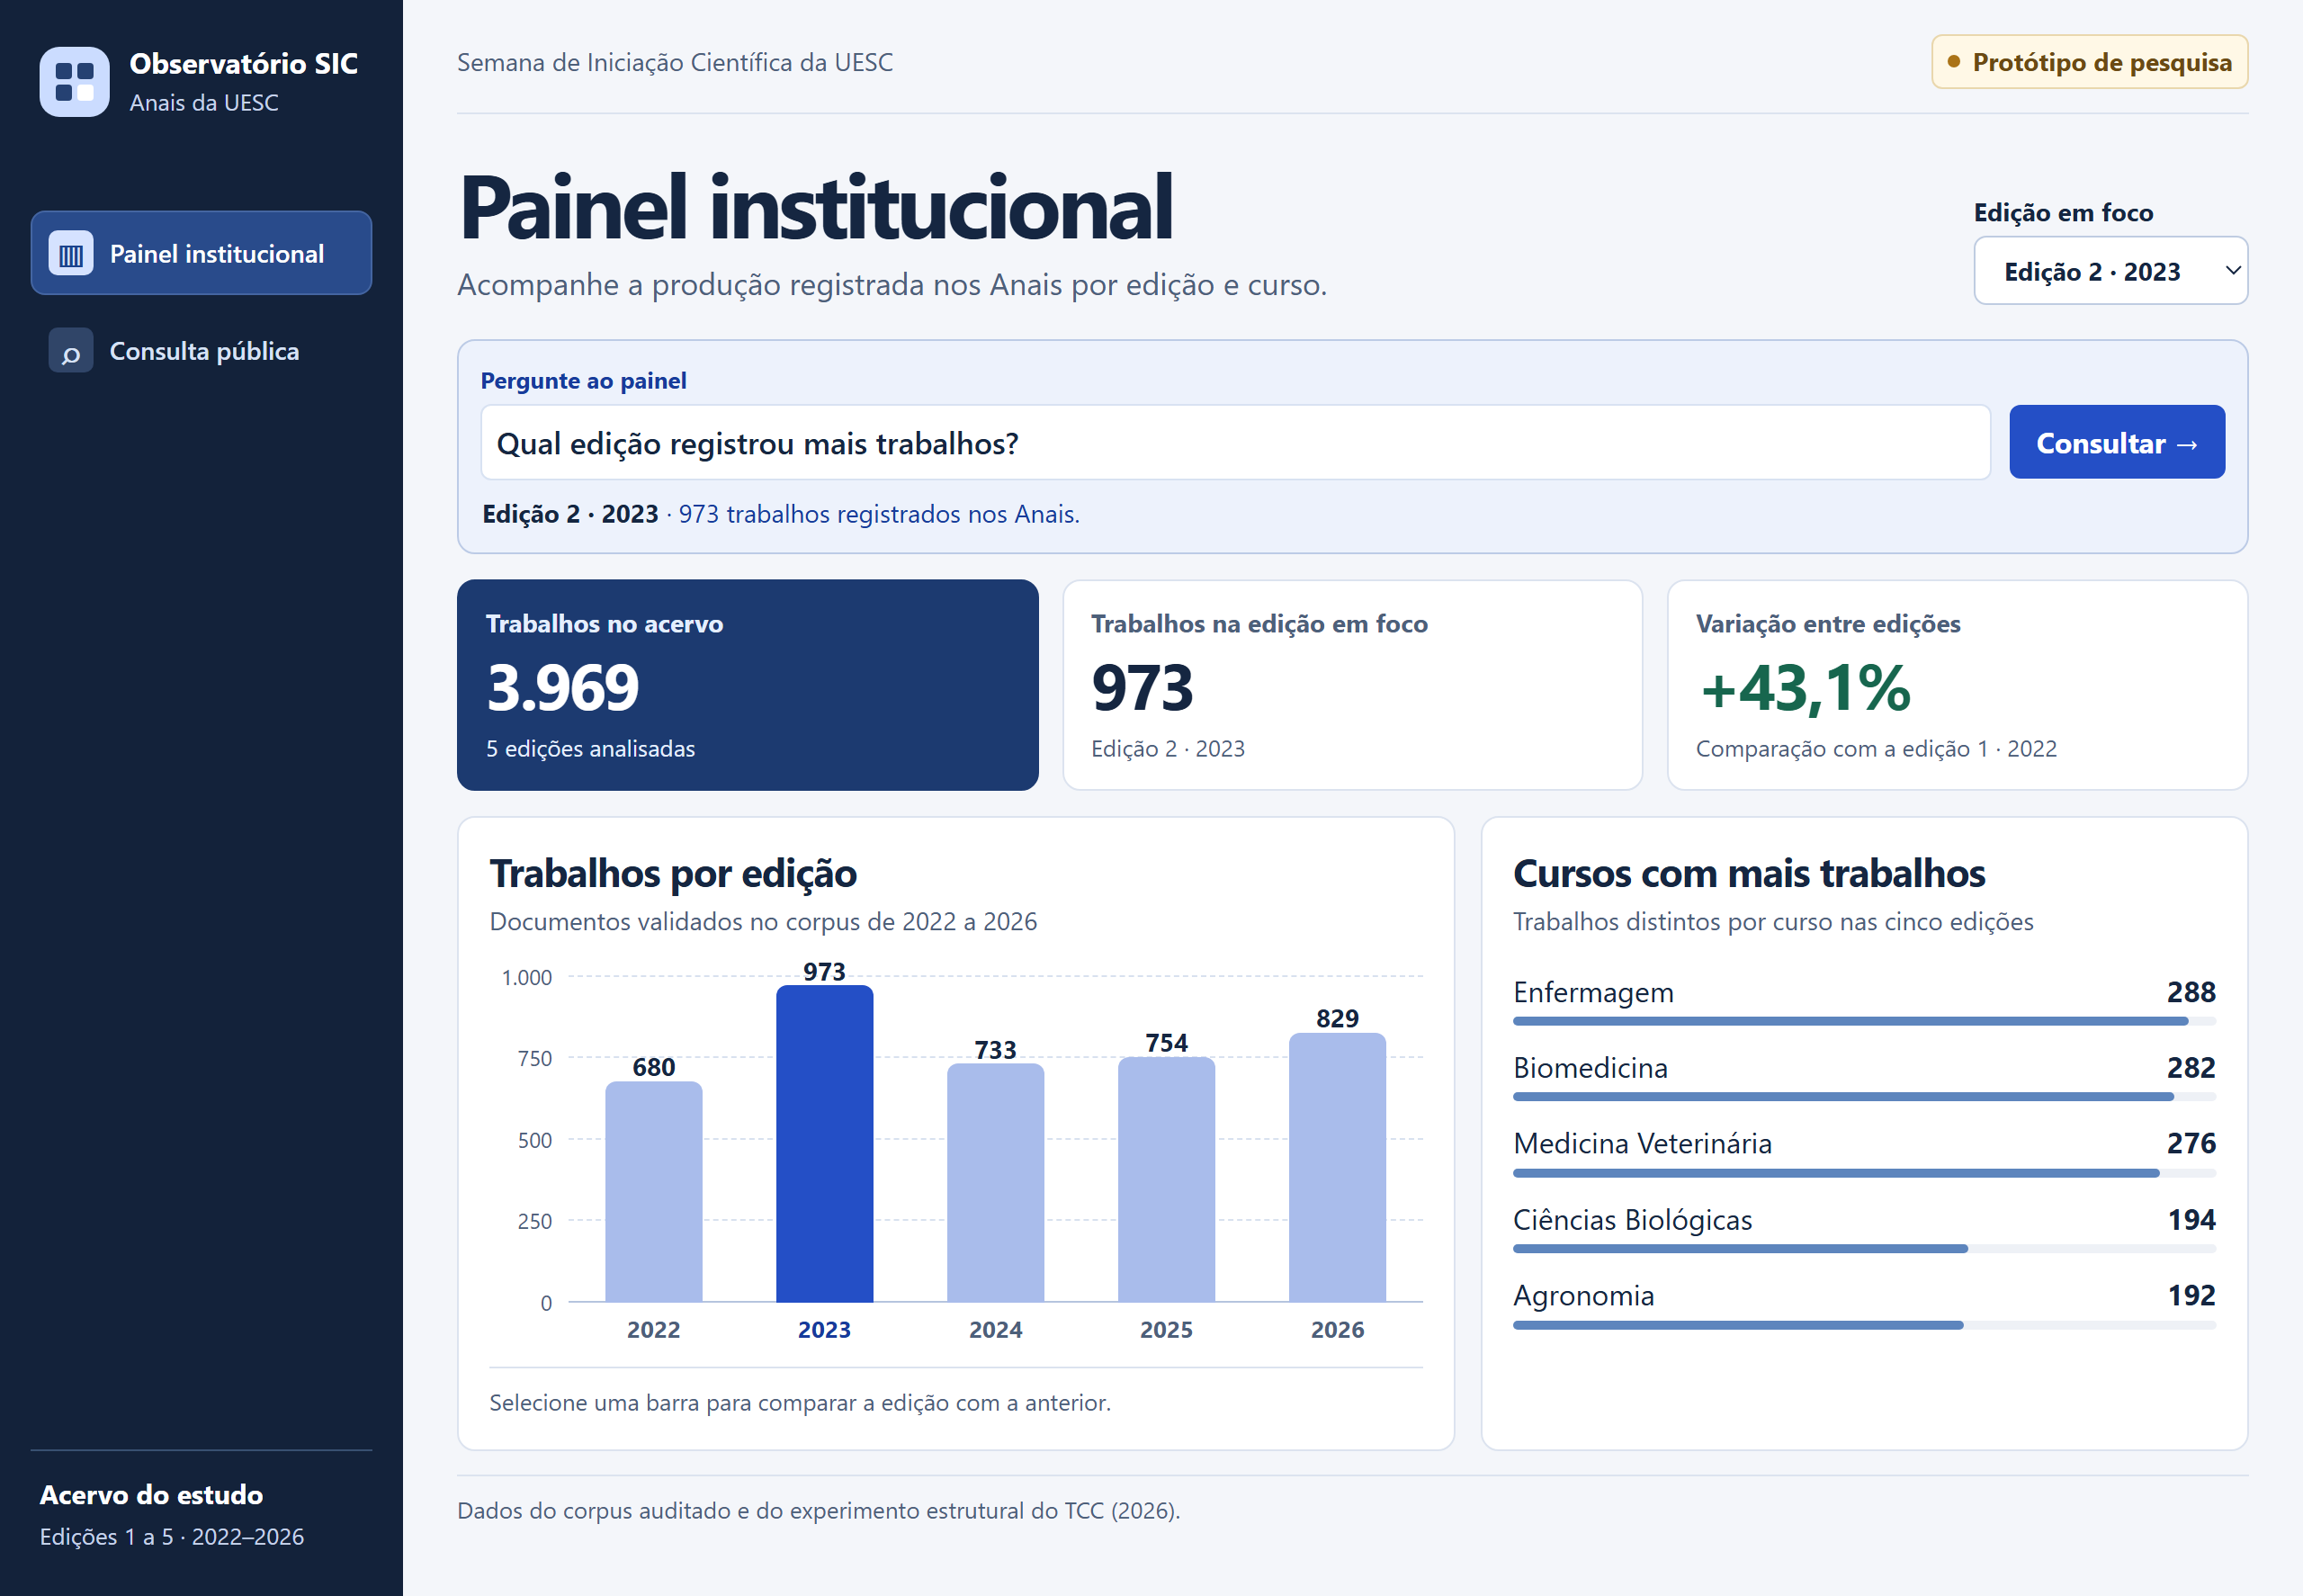
\includegraphics[width=\linewidth]{figuras/observatorio_sic_painel_institucional.png}
\par\smallskip
{\setstretch{1}\footnotesize\textbf{Fonte:} Elaborado pelo autor com dados da pesquisa (2026).\par}
\end{minipage}
\end{figure}

Também se prevê disponibilizar uma versão pública da plataforma para que estudantes, pesquisadores e demais interessados possam consultar os Anais em linguagem natural. A interface poderá facilitar a localização de trabalhos por tema, autor, orientador, curso ou edição, com referências aos documentos originais para conferência. Para estudantes, esse recurso poderá apoiar a identificação de pesquisas anteriores e de possíveis interlocutores acadêmicos. Para pesquisadores, poderá facilitar a descoberta de trabalhos correlatos e de oportunidades de colaboração.

A Figura~\ref{fig:prototipo-consulta-publica} ilustra uma consulta por autor no protótipo da interface pública. A resposta identifica os trabalhos encontrados e permite associá-los aos registros de origem nos Anais.

\begin{figure}[!htbp]
\centering
\begin{minipage}{\textwidth}
\caption{Protótipo da consulta pública em linguagem natural}
\label{fig:prototipo-consulta-publica}
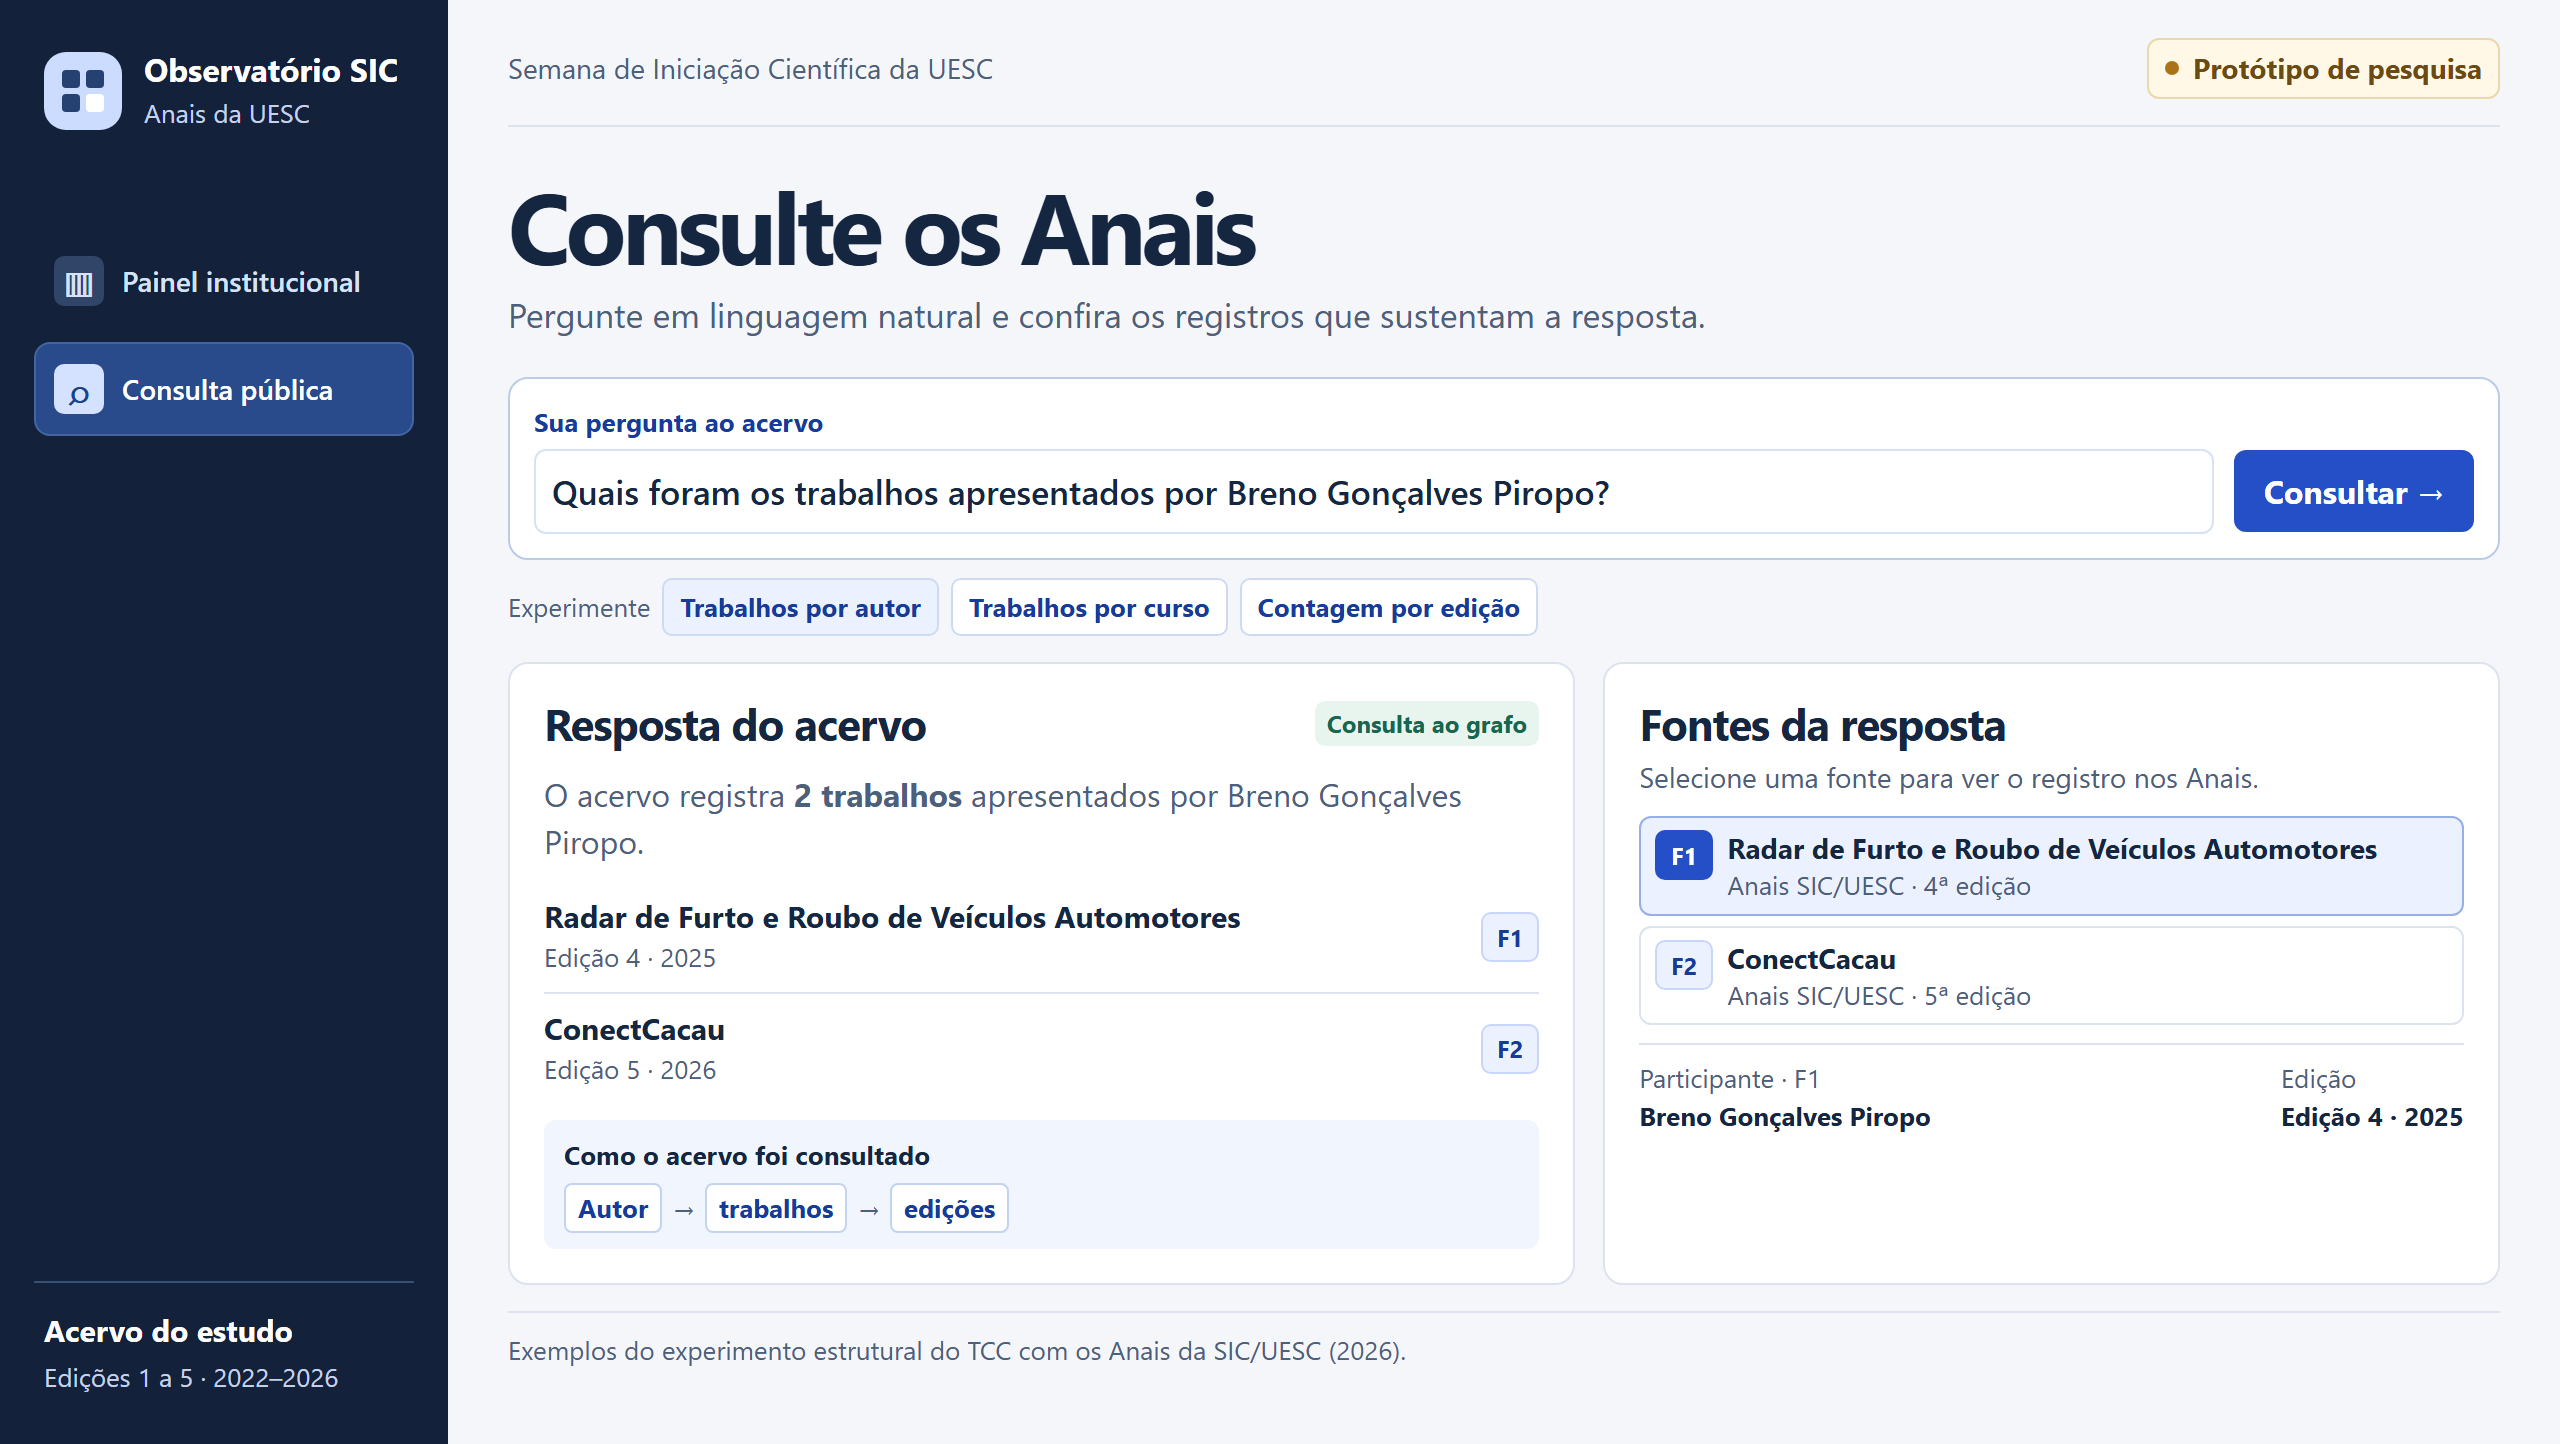
\includegraphics[width=\linewidth]{figuras/observatorio_sic_consulta_publica.png}
\par\smallskip
{\setstretch{1}\footnotesize\textbf{Fonte:} Elaborado pelo autor com dados da pesquisa (2026).\par}
\end{minipage}
\end{figure}

A incorporação de novas edições permitirá ampliar progressivamente o acervo consultável e acompanhar a evolução da produção registrada no evento. Com essas extensões, os Anais poderão servir de base tanto para a exploração pública da produção científica quanto para o planejamento de ações institucionais voltadas à iniciação científica na UESC.


\bibliographystyle{abntex2-alf}
\bibliography{biblio}

\end{document}
